%\chapter{The tidyverse and the Basics of Plotting Data}
\chapter[Harnessing Sacred Rites of the tidyverse: Plotting Basics]{Harnessing Sacred Rites of the tidyverse:\\ \huge The Basics of Plotting Data with R}

\lettrine{T}{he} history of R can be split into two epochs. There was the time before the tidyverse, a period of primordial chaos that involved much personal sacrifice and necessary violence. Then there was the time of the tidyverse. The tidyverse is a set of mystical, yet cohesive, R packages brought forth by the sorcery of Hadley Wickham and his coven of arcane programmers \parencite{Wickham2019}. 

\begin{wrapfigure}[13]{r}{0.3\textwidth}
  \begin{center}
    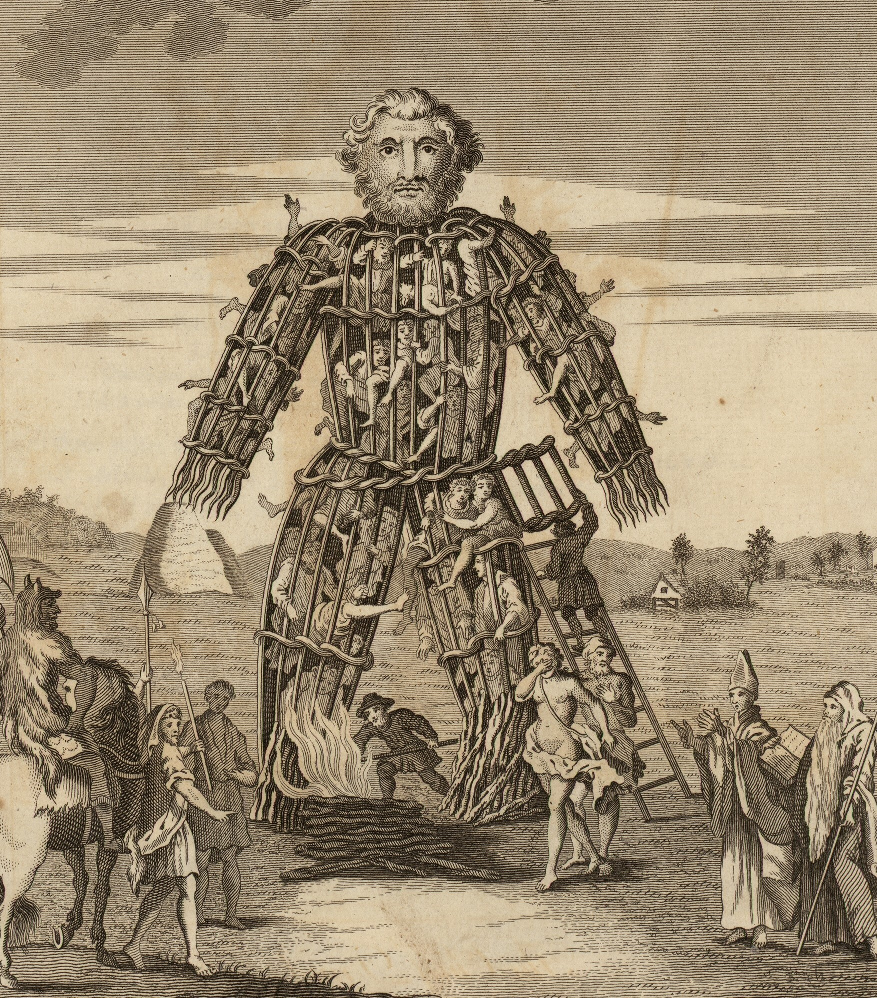
\includegraphics[width=0.28\textwidth]{graphics/ch2Figs/t_pennant.pdf}
  \end{center}
    \caption{An engraving depicting acolytes of the tidyverse burning live sacrifices, captive within a large wicker effigy, to appease their deities \parencite{Pennant1784}.}
    \label{fig:ch2_wicker}
\end{wrapfigure}


The tidyverse offers much order to the world of R, allowing common folk to bend and visualize data to their will in ways not previously possible to all but the most privileged. Though once viewed as complex and heretical \parencite{Muenchen}, through collaboration and shared learning, the dark art of \textit{tidy data} has continued to grow and flourish. While some sacrifice is inevitable (see Figure \ref{fig:ch2_wicker}), there is no denying that the tidyverse offers an unparalleled path to power, efficiency, and dark beauty in the seemingly purposeless world of data analysis. For this reason we must begin our journey into the basics of data plotting with a brief discussion of it.

% \begin{wrapfigure}[6]{r}{0.3\textwidth}
%   \begin{center}
%     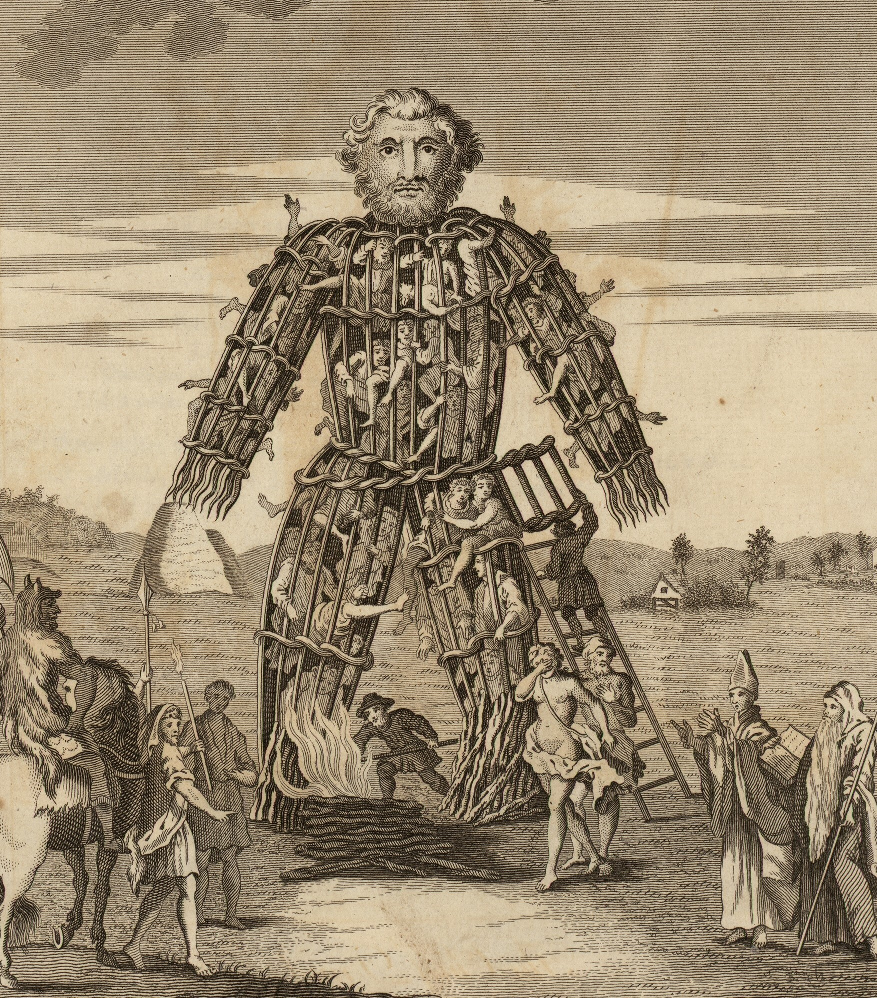
\includegraphics[width=0.3\textwidth]{graphics/ch2Figs/t_pennant.pdf}
%   \end{center}
%     \caption{An engraving depicting acolytes of the tidyverse burning live sacrifices, captive within a large wicker effigy, to appease their deities \parencite{Pennant1784}.}
%     \label{fig:ch2_wicker}
% \end{wrapfigure}

\section{Worshiping at the alter of the tidyverse}
\label{sec:tidyverse}

As described by its website (\url{https://www.tidyverse.org/}), the \gls{tidyverse} is an opinionated collection of R packages that share an underlying design philosophy. Each package can be installed individually, though most find it easiest to install every package within the scope of the tidyverse all at once.


\begin{inR}
install.packages("tidyverse")
library(tidyverse)
\end{inR}

% \begin{outR}
% -- Attaching core tidyverse packages -- tidyverse 2.0.0 --
%  dplyr     1.1.4      readr     2.1.5
%  forcats   1.0.0      stringr   1.5.1
%  ggplot2   3.5.1      tibble    3.2.1
%  lubridate 1.9.3      tidyr     1.3.1
%  purrr     1.0.2     
% -- Conflicts -------------------- tidyverse_conflicts() --
%  dplyr::filter() masks stats::filter()
%  dplyr::lag()    masks stats::lag()
%  Use the conflicted package to force all conflicts to
%  become errors
% \end{outR}

\begin{outR}
── Attaching core tidyverse packages ─────────────────────────────────────── tidyverse 2.0.0 ──
dplyr     1.1.4     readr     2.1.5
forcats   1.0.0     stringr   1.5.1
ggplot2   3.5.1     tibble    3.2.1
lubridate 1.9.3     tidyr     1.3.1
purrr     1.0.2     
── Conflicts ───────────────────────────────────────────────────────── tidyverse_conflicts() ──
dplyr::filter() masks stats::filter()
dplyr::lag()    masks stats::lag()
Use the conflicted package to force all conflicts to become errors
\end{outR}

While the above code installs all the packages, running \R{library(tidyverse)} only loads the the nine ``core'' packages:  \textit{ggplot2}, \textit{dplyr}, \textit{tidyr}, \textit{readr}, \textit{purr}, \textit{tibble}, \textit{stringr}, \textit{forcats}. Other tidyverse packages, such as \textit{readxl}, will need to be loaded separately using the \R{library()} function.

Speaking for the beginner, it will be noticed that when the tidyverse is loaded, not only is there a confirmation of what packages (and their versions) have been loaded, but there is also a list of ``conflicts'' displayed in the output.\footnote{Most packages will not display this information for you quite so nicely as the tidyverse does, so pay attention to any messages you receive using the \R{library()} function.} For instance, two functions from the \textit{dplyr} package, \R{filter()} and \R{lag()}, have the same name as pre-existing functions within R and, when you load a package with a conflict like this, precedence is always given to the most recently loaded package. This means, when you use the \R{filter()} function for example, R is going to use the version belonging to \textit{dplyr}, not the original version that was a part of base R's \textit{stats} package (which is pre-loaded each time you use R). Though you can still use that original version in the following manner: \R{package\_name::function\_name()}.  For example, \R{stats::filter()}. 

As a whole, the tidyverse will not solve all your problems, but it will come damn close. Admittedly, and this is particularly true for beginners, much of what the tidyverse offers will not be needed in your daily programming rituals, but will come in handy when least expected.

\section{Plotting with R}

A core component of any GOOD DATA ANALYSIS obviously involves visualizing your data. As you progress through the various topics in this book, specific types of plots and their uses will be discussed in detail; however, for the time being, it will be helpful to get an intuitive sense of how plotting works with R generally. Thus, what follows in this section is intended to help you understand the logic of plotting with R. The goal at this point is not to make you an expert; rather, it is to provide beginners with a base level of knowledge.

By itself, base R comes with a stock set of functions for plotting data. To illustrate we can run the following code to produce a nice looking histogram ...

\begin{inR}
x <- rnorm(10000)
hist(x)
\end{inR}
\vspace{1em}

\noindent
In the case of the above code, the function \R{rnorm()} is just generating 10,000 random values.\footnote{The random values are technically coming from a ``standard normal'' distribution (hence the ``norm'' in \R{rnorm}), but don't worry about that for now.} The function \R{hist(x)}, is simply plotting those values as a histogram.  Running the code should generate an output similar to what you see below.

\begin{figure}[H]
\centering
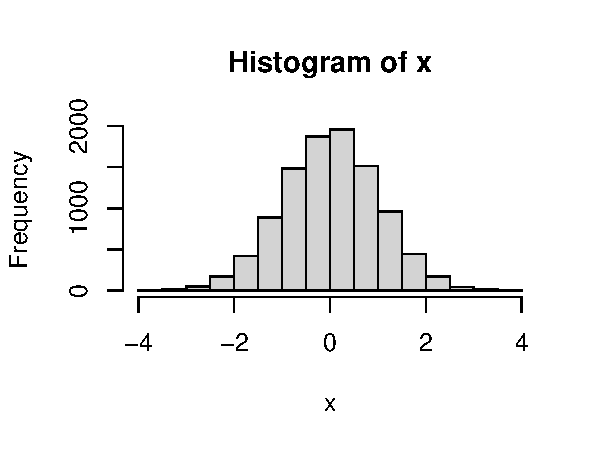
\includegraphics[scale = 0.75, trim={0 5mm 0 0},clip]{graphics/ch2Figs/base_hist.pdf}
\caption{An example of base R's plotting functions.}
\label{fig:base_hist}
\end{figure}

R's base plotting functions offer a convenient means of producing simple quality plots and can be very efficient when working with \gls{univariate data} or \gls{bivariate data}.  That is, data which consists of only one (uni) or two (bi) variables; however, most research concerned with analyzing \gls{multivariate data}. That is data with more than two variables. Each additional variable adds ever increasing amounts of complexity and nuance to your data and, by extension, the plots you use to visualizing those data.  The stock set of plotting functions R offers can accommodate these more complex scenarios; however, that level of accommodation is heavily dependent on the users proficiency with R.  For this reason, this book will adopt the practice of ignoring R's base plotting functions, and instead rely on well-known R package called \textit{ggplot2} which is among the most venerated portions of the tidyverse.   

The \textit{``gg''} in \textit{ggplot2} stands for ``grammar of graphics'' and provides users with a logical framework for the construction of plots within R.  The term ``grammar'' here is likely to conjure up long forgotten traumas of boring English and Language Arts lessons, but do not fear, the use of the term grammar is really just to emphasize that \textit{ggplot2} is constructed in a way that allows users to build plots of various kinds in a consistent and efficient manner that is easily tailored to their specific needs.  This is in contrast to how plotting in software works generally, where you are frequently stuck trying to fit a square peg (your data) into a circular hole (the software's narrow conception of how data should be presented).

The easiest way to understand how \textit{ggplot2} works is to simply dive in and use it. Along the way, we will also learn a little bit more about R and data manipulation. However, a disclaimer is perhaps useful here:

\begin{center}
    {\Huge\warning}
\end{center}

\begin{displayquote}
This chapter contains a large variety of functions and strategies for plotting data with \textit{ggplot2}. If you are under the impression that you need to memorize all of this, you are approaching this whole endeavor from the wrong angle. Programming is a skill you develop, not a collection of facts you remember (though you can foolishly treat it as such). With time and practice, your skill will improve, and you will naturally remember the various functions and methods employed in R. Eventually, you will find yourself needing to reference examples less frequently. The goal of this chapter is to help you \textbf{experience} how \textit{ggplot2} and R work. Focus on understanding the logic behind the code rather than trying to memorize it. Dive in, get your hands dirty, make mistakes, and experiment — that is how you will truly learn.
\end{displayquote}

The first thing to do will be to ensure that \textit{ggplot2} has been installed into our computer's library of packages and loaded so we can access its functions. As mentioned in section \ref{sec:tidyverse}, if you have installed and loaded the tidyverse, this is already done, but if you chose not to do that,\footnote{Shame on you.} \textit{ggplot2} can be installed and loaded as a standalone package as well.

\begin{inR}
install.packages("ggplot2")
library(ggplot2)
\end{inR}

\subsection{An example data set: msleep}

Before we can plot anything, we need something to plot.  In addition to its large set of plotting functions, the \textit{ggplot2} package also provides a few illustrative data sets.\footnote{Base R comes with a nice collection of data sets as well. To obtain a list you need only run the function \R{data()}.  To obtain the list of data sets for \R{ggplot2} you need only include the package name as an argument in this function: \R{data(package = "ggplot2")}} We will work with the \R{msleep} data set, which provides a variety of measurements relevant to the sleep behaviour of a wide range of mammals. To access the data you need only run the code \R{msleep}, which will output a $83 \times 11$ data frame.\footnote{Technically we are looking at a ``tibble'', which is the ``tidyverse's'' own take on a data frame. For our present purposes though, this is a distinction without a difference.} Given the limited space available in the console window, the data frame is going to be truncated substantially. Thus, if you would like to view the entire data set, you can utilize R's \R{View()} function, which will display the data in a separate spreadsheet style window.

\begin{inR}
msleep # print data to console
View(msleep) # view the data in a spreadsheet-style window
\end{inR}

\vspace{2em}

% latex table generated in R 4.2.1 by xtable 1.8-4 package
\begin{table}[h]
\centering
\footnotesize
\ttfamily
\begin{tabular}{rlllllr}
  \hline
 & name & genus & vore & order & conservation & sleep\_total \\ 
  \hline
1 & Cheetah & Acinonyx & carni & Carnivora & lc & 12.10 \\ 
  2 & Owl monkey & Aotus & omni & Primates &  & 17.00 \\ 
  3 & Mountain beaver & Aplodontia & herbi & Rodentia & nt & 14.40 \\ 
  4 & Greater short-tailed shrew & Blarina & omni & Soricomorpha & lc & 14.90 \\ 
  5 & Cow & Bos & herbi & Artiodactyla & domesticated & 4.00 \\ 
  6 & Three-toed sloth & Bradypus & herbi & Pilosa &  & 14.40 \\ 
  7 & Northern fur seal & Callorhinus & carni & Carnivora & vu & 8.70 \\ 
  8 & Vesper mouse & Calomys &  & Rodentia &  & 7.00 \\ 
  9 & Dog & Canis & carni & Carnivora & domesticated & 10.10 \\ 
  10 & Roe deer & Capreolus & herbi & Artiodactyla & lc & 3.00 \\ 
   \hline
\end{tabular}
\rmfamily
\caption{First 10 rows and 6 columns of the \R{msleep} data}
\label{table:msleep}
\end{table}

\noindent
Table \ref{table:msleep} shows the first 10 rows and 6 columns of \R{msleep} data.  Looking more closely at the data, we can see a variety of variables (the column names) that are, for the most part, self explanatory.
In this case, the column names represent distinct variables that have been measured and, particularly with larger data frames that cannot be adequately printed to the console, it is often useful to have R list out the name of each column. We can do this quite easily using the \R{names()} function.

\begin{inR}
names(msleep)
\end{inR}
\begin{outR}
 [1] "name"         "genus"        "vore"        
 [4] "order"        "conservation" "sleep_total" 
 [7] "sleep_rem"    "sleep_cycle"  "awake"       
[10] "brainwt"      "bodywt"   
\end{outR}

Now, while the names of each column are self-explanatory, the elements of each column are perhaps less so.  For instance, in the \R{\$sleep\_total} column, are we looking at values in minutes, hours, or days? In the \R{\$conservation} column we can see a number of abbreviations such as \R{lc}, \R{nt}, \R{vu}, and so on. What do we make of those? A good starting point for answering these questions is to check the documentation associated with the data set, which all CRAN packages are required to include. This can be accessed in the usual way with a \R{?}

\begin{inR}
?msleep
\end{inR}
\vspace{1em}

\noindent
Inspecting the documentation, we can see that \R{\$sleep\_total} is given in hours and that the column \R{\$conservation} indicates ``the conservation status of the animal.''  Admittedly, concerning this latter column, that does not tell us too much, but it does at least give us a starting point for understanding what those values might represent.  In all likelihood, we are seeing abbreviations for the IUCN's (International Union for Conservation of Nature) species ranking. 

\begin{itemize}
\setlength\itemsep{-1em}
    \item \R{lc} = Least Concern
    \item \R{nt} = Near Threatened
    \item \R{vu} = Vulnerable
    \item \R{en} = Endangered
    \item \R{cd} = Conservation Dependent
\end{itemize}

Using a \gls{scatter plot} as a basic starting point, we will plot the relationship between the variables body weight (kg) and sleep total (hours).  These are represented by the columns \R{\$bodywt} and \R{\$sleep\_total} respectively. 

\section{Adding layers}

\textit{ggplot2} constructs plots by adding visual layers on top of one another. The first layer is the grid upon which our scatter plot's points will appear.  To generate this first layer we can simply type ...

\begin{inR}
ggplot(data = msleep, aes(x = bodywt, y = sleep_total))
\end{inR}

\vspace{2em}

\begin{figure}[H]
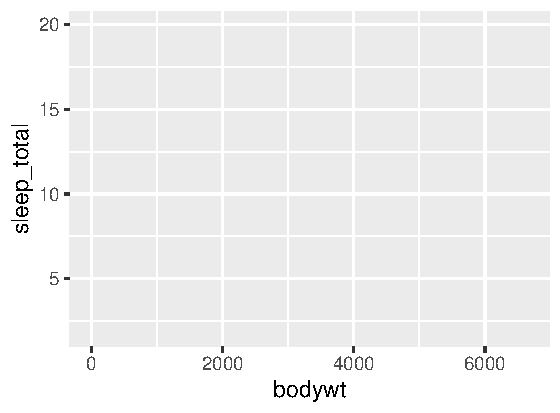
\includegraphics[scale = 0.75]{graphics/ch2Figs/ggEx_1.pdf}
\label{fig:ggEx_1.pdf}
\end{figure}

\noindent
Looking at the \R{ggplot()} function we typed, we can see that the argument \R{data} tells \textit{ggplot2} where the data is coming from - in this case it is coming from the \R{msleep} data frame.  The \R{x} and \R{y} arguments are telling \textit{ggplot2} what variables/columns should be mapped to the x and y axis respectively.  Notice that, not only has \textit{ggplot2} labelled the axis accordingly, but it has also given them scales that correspond to size of the values found in both columns.

Next we will, quite literally, add (\R{+}) a layer of points on top of this by typing \R{+ geom\_point()}. The term ``geom'' here is just an abbreviation for ``geometric object'', and points are one of many different types of geometric object \textit{ggplot2} recognizes.

\begin{inR}
ggplot(data = msleep, aes(x = bodywt, y = sleep_total)) +
  geom_point()
\end{inR}

\vspace{2em}

\begin{figure}[H]
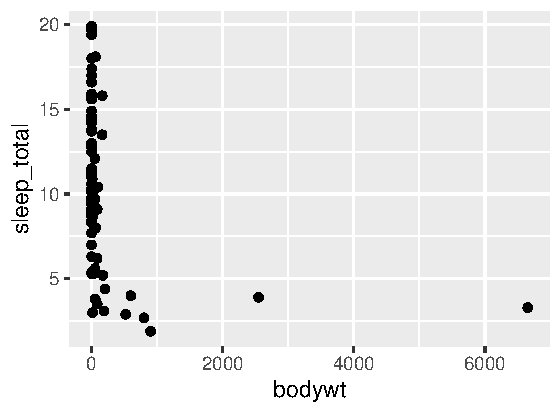
\includegraphics[scale = 0.75]{graphics/ch2Figs/ggEx_2.pdf}
\label{fig:ggEx_2.pdf}
\end{figure}

\noindent
At this juncture, it is worth taking a moment to talk about how this code we have written has been organized. Here we placed \R{geom\_point()} on a new line and indented it.  This was not something we strictly had to do.  We could have put everything on a single line like so ...

\begin{inR}
ggplot(data = msleep, aes(x = bodywt, y = sleep_total)) + geom_point()
\end{inR}

\vspace{1em}

\noindent
But, particularly as we add more customization to the plot, this style of writing becomes hard to read. The (tidyverse's) \href{https://style.tidyverse.org/syntax.html#long-lines}{R style guide} recommends that no line of code exceed 80 characters, which is the advice most of the R community adheres to. In fact, Rstudio can be configured to display a margin representing the 80 character limit: (\textit{Tools $\rightarrow$ Global Options $\rightarrow$ Code $\rightarrow$ Display}). To ensure that you do not exceed limit with larger blocks of code, it is worth remembering that you can always move portions of code to a new line after a comma, operator, or unclosed parentheses. The indentation we used is purely to guide the eye in recognizing that \R{geom\_point()} belongs to a larger block of code.\footnote{While the R programming language allows users to indent code with reckless abandon, some programming languages, such as \textit{Python}, require it to be used in very specific ways.}

\subsection{Inspecting potential outliers}

At present, the plot does not look like much.  There are numerous points scattered between 0 and 1000, and a couple of very extreme points beyond which are skewing the x-axis scale and making the majority of the data difficult to visualize. Given how rare and extreme these two values appear, we should inspect them to ensure that they are not errors within the data set (i.e., ensure that there is not a 2500 kg mouse, bird, or other such abomination in our data set). To accomplish this, most people will instinctively try to scan the data frame's 83 rows one by one with their eyes. Obviously, that strategy will be slow, inefficient, and highly prone to error.  A better strategy is to have R isolate these values using the \R{filter()} function which is part of the tidyverse's \textit{dplyr} package.\footnote{Base R has a (more or less) equivalent function \R{subset()} that we could use as well. There are reasons for preferring \R{filter()}, but in this context there is no advantage to using either.}  We simply give the function our data frame, and then specify a logical rule to subset by. In this case we will tell the function to show us all the rows that have a body weight greater than 2000.

\begin{inR}
filter(msleep, bodywt > 2000)
\end{inR}

\begin{outR}
# A tibble: 2 × 11
  name             genus     vore  order       conservation sleep_total
  <chr>            <chr>     <chr> <chr>       <chr>              <dbl>
1 Asian elephant   Elephas   herbi Proboscidea en                   3.9
2 African elephant Loxodonta herbi Proboscidea vu                   3.3
# 5 more variables: sleep_rem <dbl>, sleep_cycle <dbl>, awake <dbl>, 
# brainwt <dbl>, bodywt <dbl>
\end{outR}

\vspace{1em}

A quick glance at the output reveals that these two points represent the Asian and African elephant respectively.  Thus, while these values are quite extreme and do not seem to be terribly representative of the data as a whole, they are not mistakes and therefore should remain in the data set.  However, this begs the question, how do we visualize this data adequately with such odd scaling?

\subsection{Logarithms}

A common strategy in cases like this where larger values tend to become more and more extreme (i.e., exhibit some kind of exponential growth) is to plot the logarithm of the values. As a refresher of high school mathematics, logarithms are essentially exponents in reverse. For example:

\vspace{-2em}

$$10^3 = 10 \times 10 \times 10 = 1000$$

\vspace{-1em}

\noindent
A \textit{base-10} logarithm simply undoes this process by stating how many 10s it takes to create 1000.

\vspace{-2em}

$$\log_{10}(1000) = 3$$

\vspace{-1em}

\noindent
A \textit{base-2} logarithm asks: how many 2s are required to create 1000?

\vspace{-2em}

$$\log_{2}(1000) \approx 9.966$$

\vspace{-1em}

\noindent
Thus, $2^{9.966} \approx 1000$.  

%\vspace{-1em}

\noindent
A \textit{natural} logarithm uses a base denoted as $e$ (Euler's Number), which is approximately 2.71828.

\vspace{-2em}

$$\log_e(1000) \approx 6.908$$

\vspace{-1em}

\noindent
Base-10, base-2, and natural logarithms represent the most widely used types of logarithms,\footnote{For clarity and consistency the natural logarithm of 1000 has been written $\log_e(1000)$, but it is common practice to identify natural logarithms using ``$\ln$''. E.g., $\ln{(1000) \approx 6.908}$.} but you can technically use any base you desire.  As seen below, the use of logarithms in R is very straightforward.

\begin{inR}
log10(1000) # Base-10 function
log2(1000) # Base-2 function
log(1000) # Natural log
log(1000, base = 666) # Pick your own base
\end{inR}
\begin{outR}
[1] 3
[1] 9.965784
[1] 6.907755
[1] 1.062521
\end{outR}

A base-10 logarithm is generally considered the most intuitive so we will use that. There are various ways to incorporate a logarithmic scale on our plot's axis, but perhaps the safest way is to simply add a new column of $\log_{10}$ values to our dataframe and plot that instead of the standard \R{\$bodywt} column.

\begin{inR}
# Add new column of log bodywt values.
msleep$bodywt_log10 <- log10(msleep$bodywt)

# Re-plot the data
ggplot(msleep, aes(x = bodywt_log10, y = sleep_total)) +
  geom_point()
\end{inR}

\vspace{2em}

\begin{figure}[H]
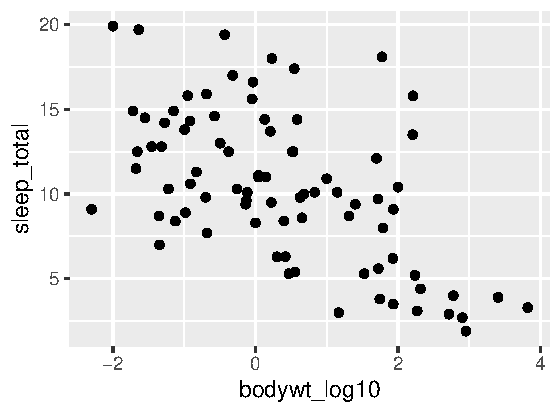
\includegraphics[scale = 0.75]{graphics/ch2Figs/ggEx_3.pdf}
\label{fig:ggEx_3.pdf}
\end{figure}

\begin{figure}[h]
    \centering
\begin{mdframed}[style = miscFrame, frametitle = Box 2.1: An alternative way to scale]

In the previous example, the logarithm was applied by creating a new column of x-axis values and plotting that. However, this means that, if you want to interpret the numbers in their original units, you need to calculate  $10^x$, which can be annoying.  

\vspace{1em}

An alternative strategy would be to keep the \R{\$bodywt} column as is and just scale the plot's axis itself to increment logarithmically which \R{ggplot2} will do straightforwardly.

\begin{inR}
ggplot(msleep, aes(x = bodywt, y = sleep_total)) +
  geom_point() +
  scale_x_continuous(trans = "log10")
\end{inR}

\vspace{4em}
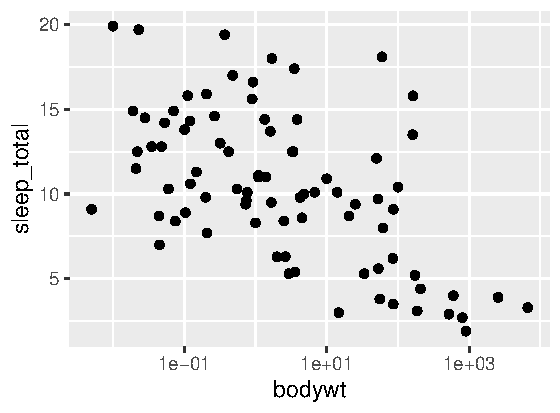
\includegraphics[scale = 0.7]{graphics/ch2Figs/ggEx_4.pdf}

\vspace{1em}

The advantage of this method is you can look at a point's value on the x-axis and know immediately that it corresponds to a weight of $x$ kg. The drawback is you may end up with excessively small or large values on the axis, hence the \href{https://www.mathsisfun.com/numbers/scientific-notation.html}{\textit{scientific notation}} you see in the plot.

\end{mdframed}
\end{figure}

\section{Aesthetics}

Geometric objects in \textit{ggplot2}, like the point geom, all have various traits, like their size, shape, and colour that can be customized.  In the language of \textit{ggplot2}, these are referred to as \gls{aesthetics}.  For example, we can customize the points in the following way ...

\begin{inR}
ggplot(msleep, aes(x = bodywt_log10, y = sleep_total)) +
  geom_point(size = 3, 
             shape = 4, 
             colour = "blue", 
             stroke = 1.5)
\end{inR}

\vspace{2em}

\begin{figure}[H]
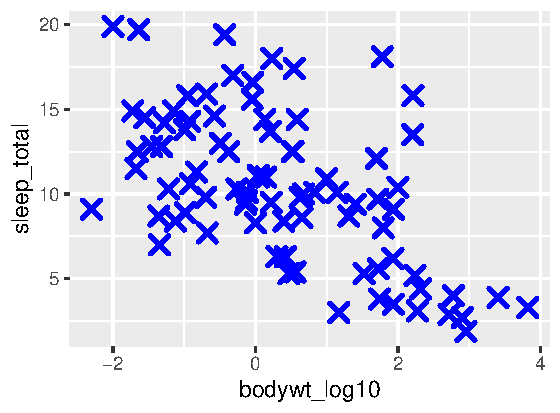
\includegraphics[scale = 0.75]{graphics/ch2Figs/ggEx_5.pdf}
\end{figure}

With a bit of experimentation, it should be apparent how the arguments \R{size} and \R{stroke} work in the above example; however, the \R{shape} and \R{colour} arguments are slightly less intuitive.\footnote{If you accidentally omit the ``u'' when typing ``colour,'' \textit{ggplot2} will still understand what you mean, even though it isn't correct English.} R comes with a variety of point shapes (technically called ``plotting characters'' or ``\gls{pch}'' symbols for short) that are denoted by numbers. The various possibilities are depicted in Figure \ref{fig:points.pdf}.  In this case, number 4 is an $\times$.  Notably, the last five plotting characters (21 through 25) incorporate both a \R{colour} aesthetic for their edges and a \R{fill} aesthetic. All the other symbols only require a \R{colour} aesthetic to be specified.

\begin{inR}
ggplot(msleep, aes(x = bodywt_log10, y = sleep_total)) +
  geom_point(
    size = 3,
    shape = 25,
    colour = "black",
    stroke = 1.5,
    fill = "red"
  )
\end{inR}

\vspace{2em}

\begin{figure}[H]
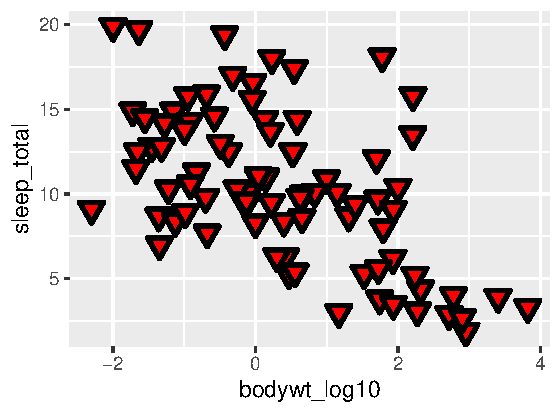
\includegraphics[scale = 0.75]{graphics/ch2Figs/ggEx_6.pdf}
\end{figure}

\noindent
The plotting characters shown in Figure \ref{fig:points.pdf} are just a few of the options available. For instance, by using values ranging between 32 and 127, you can display a variety of ASCII characters. Additionally, you can specify a particular character instead of providing a numeric value, e.g., \R{shape = "\&"}.

\vspace{2em}

\begin{figure}[h]
\centering
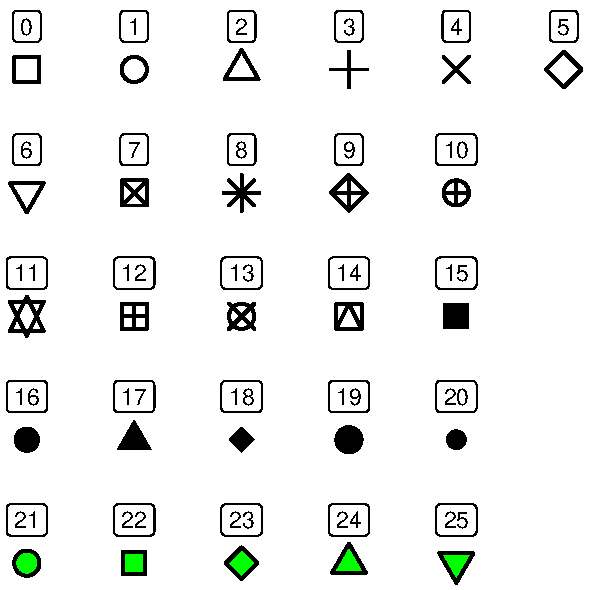
\includegraphics[scale = 0.75]{graphics/ch2Figs/points.pdf}
\caption{R Plotting Characters}
\label{fig:points.pdf}
\end{figure}

\vspace{2em}

\noindent
In the above examples we specified a desired colour by typing the name of a primary colour, but we are not limited to just using primary colours. R comes with a built in set of 657 differently named colours.  You can obtain the full list of colour names by running \R{colors()}.  R also has a built-in demo of these colours you can run to get a visual representation of each.  Simply run the command \R{demo("colors")}. 

Alternatively, instead of typing a colour name, you can use a hexadecimal value (also referred to as a ``hex code'' or ``hex value'') that represents a specific colour. For example, the hex value \R{"\#FFC0CB"} represents the colour pink. Hexadecimal values offer the user a lot of nuance when it comes to colour selection and, in most cases, the simplest way of finding an appropriate hex value is to consult one of the many websites devoted to colour codes and colour theory (i.e., do an internet search). However, if you would like to understand the theory behind hex codes and why they are used, see Box 2.2.

\begin{figure}
    \centering
\begin{mdframed}[style = miscFrame, frametitle = Box 2.2: Hexadecimal Notation for Colours]

Hexadecimal values are simply numbers that use a base-16 counting method. In other words, in the world of hexadecimals, there are 16 different numbers that are used to count with, instead of the typical 10 numbers (0:9), you were probably raised to use. These are 

\vspace{1em}

\begin{table}[H]
\centering
\begin{tabular}{|l|l|l|l|l|l|l|l|l|l|l|l|l|l|l|l|l|}
\hline
\textbf{Decimal}     & 0 & 1 & 2 & 3 & 4 & 5 & 6 & 7 & 8 & 9 & 10 & 11 & 12 & 13 & 14 & 15 \\ \hline
\textbf{Hexadecimal} & 0 & 1 & 2 & 3 & 4 & 5 & 6 & 7 & 8 & 9 & A  & B  & C  & D  & E  & F  \\ \hline
\end{tabular}
\end{table}

\vspace{1em}

\noindent
Because of their larger base, a single hexadecimal digit can store more information than a conventional base-10 digit can.  For instance, if a computer stores various gradations of the colour red using just two digits, that only allows for 100 ($10 \times 10$) different reds. Using hexadecimals you can have 256 ($16 \times 16$) reds, with just two digits.  Thus, if a colour is some combination of red, green, and blue, and each is stored using two hexadecimal digits that gives you $256^3 = 16,777,216$ colours as opposed to the meagre $100^3 = 1,000,000$ you would have using the inferior base-10 counting method.

\vspace{1em}

To use hexadecimals to represent colour, two digits are assigned to red (RR), green (GG) and blue (BB), in that order like so \R{"\#RRGGBB"}.  Smaller values are darker, and larger values are brighter.  Consequently, black is represented as \R{"\#000000"} and white is represented as \R{"\#FFFFFF"}. Thus, if you want the ``purest'' red, you would input \R{"\#FF0000"}, the purest green would be \R{"\#00FF00"}, and the purest blue would be \R{"\#0000FF"}.
\end{mdframed}
\end{figure}

\subsection{Aesthetics by variable}

In the above examples, the aesthetic changes we made to the plots affected all of the points. In the language of \textit{ggplot2}, we would say that the aesthetics were mapped to all the points. However, it is often necessary to visually break up the points according to one of the other variables in your data.  For instance, we could colour the points in our plot according to the categories in the data's \R{\$vore} column.

\begin{inR}
ggplot(msleep, aes(x = bodywt_log10, y = sleep_total)) +
    geom_point(size = 3, aes(colour = vore))
\end{inR}

\vspace{2em}

\begin{figure}[H]
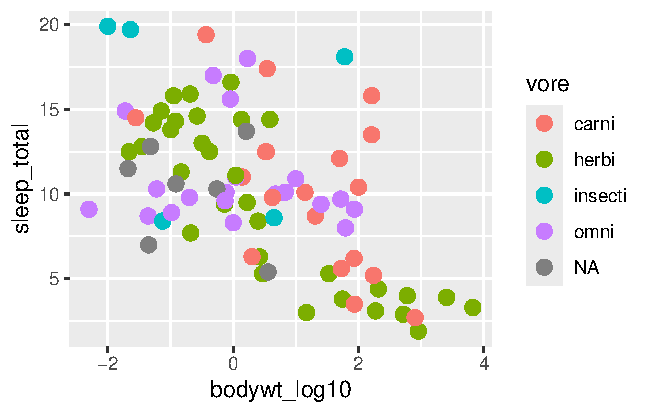
\includegraphics[scale = 0.75]{graphics/ch2Figs/ggEx_7.pdf}
\end{figure}

\noindent
Notice that the plot's legend shows an ``NA'' category. This is because there are \R{NA} values found within the \R{\$vore} column (run \R{msleep\$vore} to see them). Thus, the legend's ``NA'' category represents values that we have body weight and sleep total information for, but we do not know what those animals diet consists of and therefore cannot categorize them properly.\footnote{To see the full list of animals who have a missing \R{\$vore} value, you can run \R{filter(msleep, is.na(vore))}. This will show all the rows for which \R{is.na(vore)} evaluates to \R{TRUE}.} So instead of referring to this category as ``NA'', we could refer to these as ``unknown.'' All we need to do is change the \R{NA} values in the data frame's \R{\$vore} column to character values that read \R{"unknown"}. This can be done simply by using the \R{ifelse()} function, which tests a statement you write. If that statement is true, it produces a value you have specified, if it false, then it produces an alternative value you have specified.  In other words, it works like this: 

\noindent
\R{ifelse(test, \textit{true result}, \textit{false result})}.

\noindent
In this case, we want to test \textit{if} the value in each row \textit{is} an \R{NA} value or not. Recall that the function \R{is.na()} tells us whether the value of a vector is an \R{NA} value or not.

\begin{inR}
is.na(msleep$vore)
\end{inR}
\begin{outR}
 [1] FALSE FALSE FALSE FALSE FALSE FALSE FALSE
 [8]  TRUE FALSE FALSE FALSE FALSE FALSE FALSE
 [15] ...
\end{outR}

\noindent
Thus, we can use that as the ``test'' in the \R{ifelse()} function.

\begin{inR}
ifelse(is.na(msleep$vore), "unknown", msleep$vore)
\end{inR}

\begin{outR}
 [1] "carni"   "omni"    "herbi"   "omni"    "herbi"   "herbi"   "carni"  
 [8] "unknown" "carni"   "herbi"   "herbi"   "herbi"   "omni"    "herbi"  
[15] "omni"    "omni"    "omni"    "carni"   "herbi"   "omni"    "herbi"  
[22] "insecti" "herbi"   "herbi"   "omni"    "omni"    "herbi"   "carni"  
[29] "omni"    "herbi"   "carni"   "carni"   "herbi"   "omni"    "herbi"  
[36] "herbi"   "carni"   "omni"    "herbi"   "herbi"   "herbi"   "herbi"  
[43] "insecti" "herbi"   "carni"   "herbi"   "carni"   "herbi"   "herbi"  
[50] "omni"    "carni"   "carni"   "carni"   "omni"    "unknown" "omni"   
[57] "unknown" "unknown" "carni"   "carni"   "herbi"   "insecti" "unknown"
[64] "herbi"   "omni"    "omni"    "insecti" "herbi"   "unknown" "herbi"  
[71] "herbi"   "herbi"   "unknown" "omni"    "insecti" "herbi"   "herbi"  
[78] "omni"    "omni"    "carni"   "carni"   "carni"   "carni"  
\end{outR}

When you run the above code, the \R{ifelse()} function scans each row of the \R{\$vore} column and evaluates whether \R{is.na(msleep\$vore)} is \R{TRUE}. If it is true, it replaces the existing \R{NA} value with \R{"unknown"}. However, if it \R{FALSE}, it leaves it as the original value (this is why we wrote \R{msleep\$vore} after the second comma). The end result is a vector of values that we can use to replace the existing \R{\$vore} column with.

\begin{inR}
msleep$vore <- ifelse(is.na(msleep$vore), "unknown", msleep$vore)
\end{inR}

\vspace{1em}

\noindent
Now, when we re-plot the graph, we get something much more sensible ....

\begin{inR}
ggplot(msleep, aes(x = bodywt_log10, y = sleep_total)) +
    geom_point(size = 3, aes(colour = vore))
\end{inR}
\vspace{2em}
\begin{figure}[H]
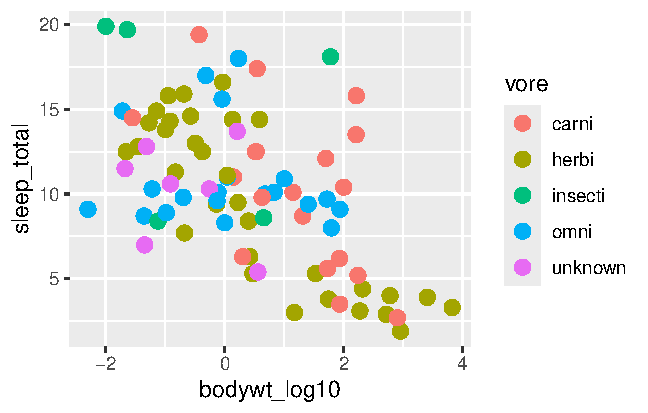
\includegraphics[scale = 0.75]{graphics/ch2Figs/ggEx_8.pdf}
\end{figure}

When plotting, it is usually inadvisable to \textit{only} adjust the colour of your points because a sizeable portion of the population has some form of colour vision deficiency (a.k.a., colour blindness). And while there are ``colourblind friendly'' palettes we can use, there is no universal palette that works optimally for all cases of colour deficiency. Consequently, the best practice is to have each category be represented by a distinct shape. 

\begin{inR}
ggplot(msleep, aes(x = bodywt_log10, y = sleep_total)) +
    geom_point(size = 3, aes(colour = vore, shape = vore))
\end{inR}

\vspace{2em}

\begin{figure}[H]
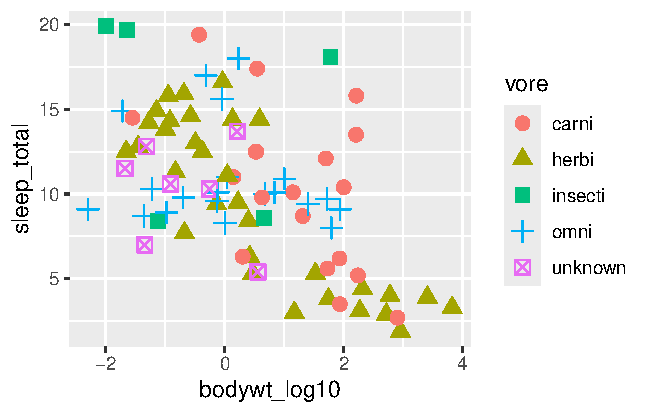
\includegraphics[scale = 0.75]{graphics/ch2Figs/ggEx_9.pdf}
\end{figure}

\section{Displaying trends}

Notice that the data points appear to trend downward as you move from left to right on the x-axis. In other words, as body weight increases, you tend to see decreases in sleep total. By simply adding a second geom, called \R{geom\_smooth()}, we can use a line of best fit to represent (i.e., model) this trend.

\begin{inR}
ggplot(msleep, aes(x = bodywt_log10, y = sleep_total)) +
    geom_point(size = 3, aes(colour = vore, shape = vore)) +
    geom_smooth()
\end{inR}
\vspace{2em}
\begin{figure}[H]
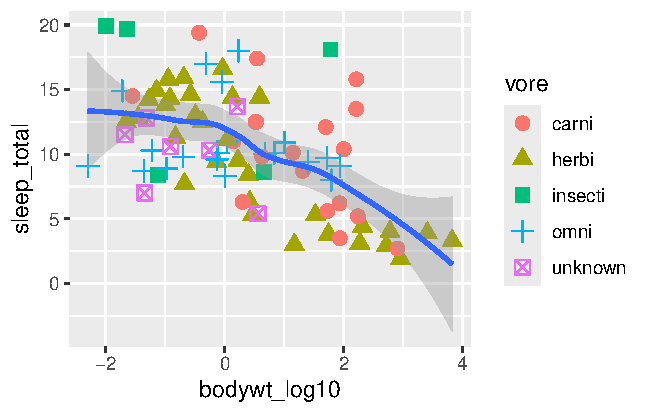
\includegraphics[scale = 0.75]{graphics/ch2Figs/ggEx_10.pdf}
\end{figure}

The shaded grey area represents a statistic called the \textit{standard error} and the line was drawn using a fancy smoothing method called \textit{local polynomial regression fitting}, but we can use a more common regression line as well and modify various aspects of it just like we had done earlier using \R{geom\_point()}.

\begin{inR}
ggplot(msleep, aes(x = bodywt_log10, y = sleep_total)) +
  geom_point(size = 3, aes(colour = vore, shape = vore)) +
  geom_smooth(
    method = "lm", se = FALSE,
    linetype = 2,
    linewidth = 0.5,
    colour = "black"
  )
\end{inR}

\vspace{2em}

\begin{figure}[H]
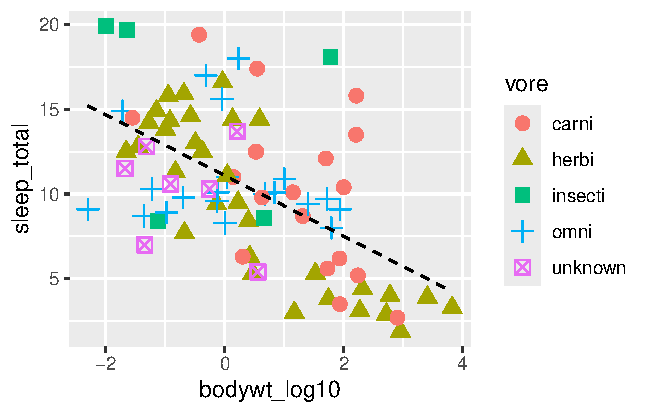
\includegraphics[scale = 0.75]{graphics/ch2Figs/ggEx_11.pdf}
\end{figure}

\noindent By setting \R{method = "lm"} on line 4, we are instructing \textit{ggplot2} to draw a linear model. While the concepts of standard error, polynomial regression, and linear models are more advanced topics, their value in displaying trends should be clear enough, even if the underlying mathematics is not yet fully understood.


It is at this point where the versatility of the \textit{ggplot2} really begins to shine.  For instance, if we wanted to create a separate regression line for each category of \R{\$vore} we can accomplish that by once again making use of the \R{aes()} function and ``grouping'' by \R{\$vore}.

\begin{inR}
ggplot(msleep, aes(x = bodywt_log10, y = sleep_total)) +
  geom_point(size = 3, aes(colour = vore, shape = vore)) +
  geom_smooth(
    method = "lm",
    se = FALSE,
    colour = "black",
    linewidth = 0.5,
    aes(group = vore)
  )
\end{inR}

\vspace{2em}

\begin{figure}[H]
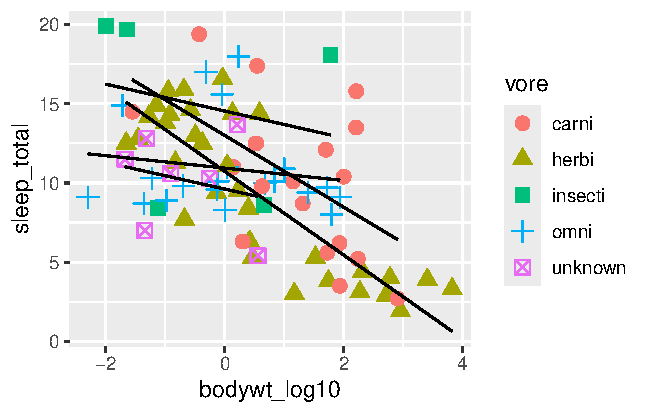
\includegraphics[scale = 0.75]{graphics/ch2Figs/ggEx_12.pdf}
\end{figure}

At present it is not clear which line applies to which category, but we could also have each regression line correspond to the colour mapped to \R{\$vore}, and (in consideration of colour blindness) give each line a separate \R{linetype}.

\begin{inR}
ggplot(msleep, aes(x = bodywt_log10, y = sleep_total)) +
  geom_point(size = 3, aes(colour = vore, shape = vore)) +
  geom_smooth(
    method = "lm",
    se = FALSE,
    linewidth = 0.5,
    aes(colour = vore, linetype = vore)
    )
\end{inR}

\vspace{2em}

\begin{figure}[H]
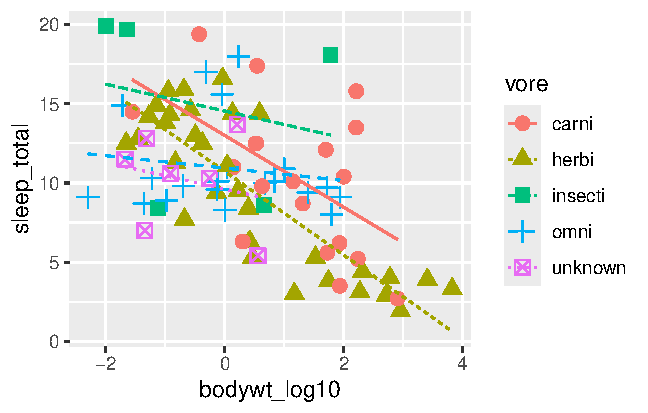
\includegraphics[scale = 0.75]{graphics/ch2Figs/ggEx_13.pdf}
\end{figure}

\section{Facets}
\label{sec:facets}

As interesting as our plot looks, it is becoming rather cluttered and difficult to visually parse. In situations like this, it is often helpful to split the plot up into separate facets (i.e., give each category its own graph). \textit{ggplot2} makes this very easy with its \R{facet\_wrap()} function.

\begin{inR}
ggplot(msleep, aes(x = bodywt_log10, y = sleep_total)) +
  geom_point(size = 3, aes(colour = vore, shape = vore)) +
  geom_smooth(
    method = "lm", 
    se = FALSE,
    linewidth = 0.5,
    aes(colour = vore)
  ) +
    facet_wrap(~ vore)
\end{inR}
\vspace{2em}
\begin{figure}[H]
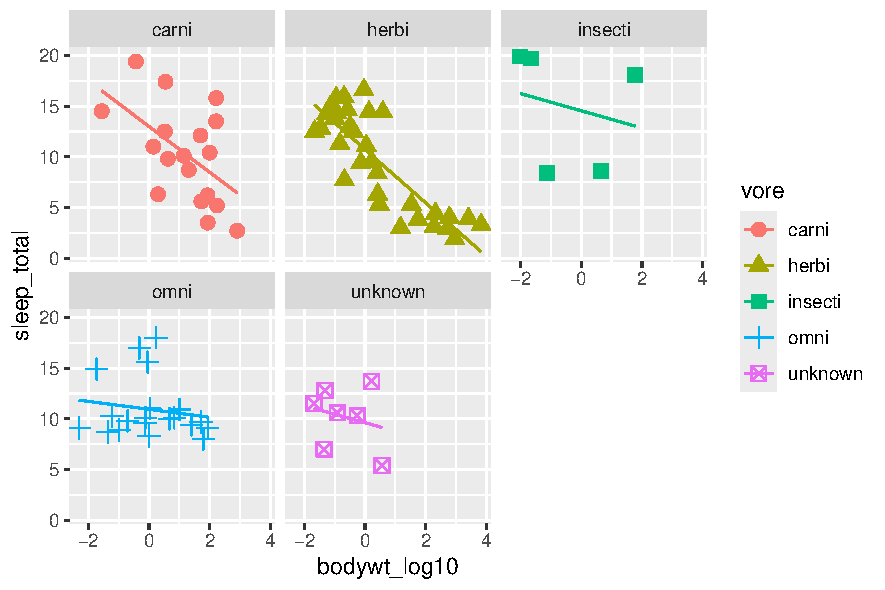
\includegraphics[scale = 0.75]{graphics/ch2Figs/ggEx_14.pdf}
\end{figure}

You can interpret the small formula we wrote (\R{\textasciitilde vore}) as meaning ``\textit{plot as a function of vore}.''

Notice that now, the colour and shape aesthetics are providing redundant information with the facet labels. As a general rule, you want to avoid redundancy in your plots because additional visual elements might bias the viewer's eye in unpredictable ways. We can easily fix this by removing some of the aesthetics we added earlier, and we can also adjust the facets so that they are all on a single row by adding the argument, \R{nrow = 1} to our \R{facet\_wrap()} function.

\begin{inR}
ggplot(msleep, aes(x = bodywt_log10, y = sleep_total)) +
  geom_point(size = 3) +
  geom_smooth(method = "lm", se = FALSE, linewidth = 0.5) +
  facet_wrap(~ vore, nrow = 1)
\end{inR}

\vspace{2em}

\begin{figure}[H]
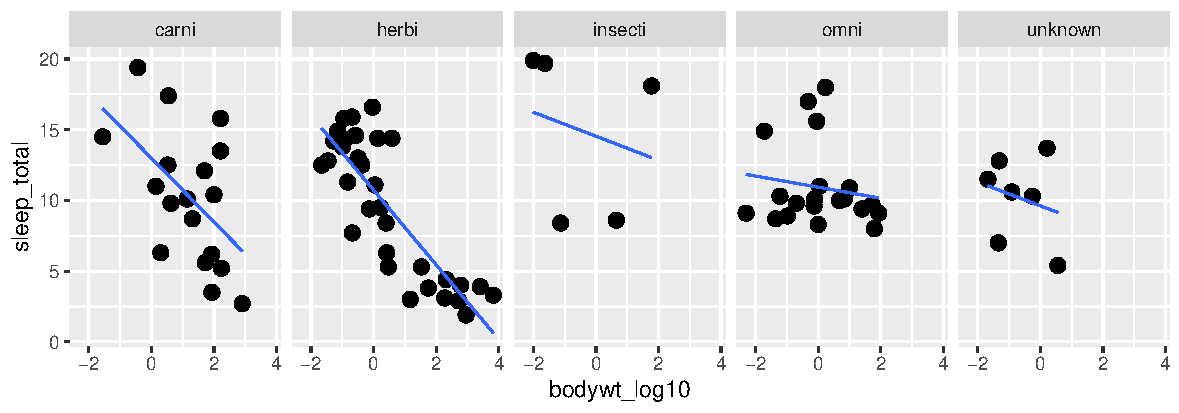
\includegraphics[scale = .75]{graphics/ch2Figs/ggEx_15.pdf}
\end{figure}

The default behaviour of \R{facet\_wrap()} preserves the x and y axis scales across the facets, making them easy to compare. In most cases, this is a feature you do not want to override but it can be done (see the R documentation: \R{?facet\_wrap}).

Particularly for beginners with R, it is difficult to impress how useful \textit{ggplot2} is here. Using base R plotting functions to produce a comparable graph would be a considerably more complex process and require a heftier amount of code to be written, whereas ggplot does it all for us in four short lines.

To finish up the plot, we should adjust some of the labelling, save it, and then take a look at some other more advanced features of \textit{ggplot2}.

\section{Labels}

To adjust the x and y axis titles we can simply use the functions \R{xlab()} and \R{ylab()}.

\begin{inR}
ggplot(msleep, aes(x = bodywt_log10, y = sleep_total)) +
  geom_point(size = 3) +
  geom_smooth(
    method = "lm",
    se = FALSE,
    linewidth = 0.5
  ) +
  facet_wrap(~vore, nrow = 1) +
  xlab("Log10(Body Weight kg)") + 
  ylab("Sleep Total (hrs)")
\end{inR}

\vspace{2em}

\begin{figure}[H]
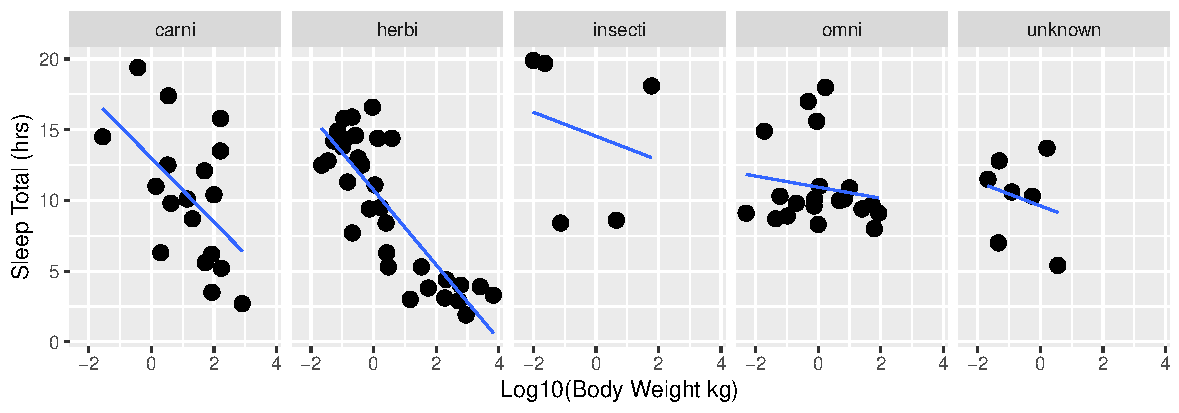
\includegraphics[scale = .75]{graphics/ch2Figs/ggEx_16.pdf}
\end{figure}

\section{Saving the plot}

Users of R studio will notice that in the \textit{Plots} pane there is a button that can be used to ``export'' your plot. However, it is usually more efficient and useful to save the plot via written code, and there are different methods you could use to go about this.  Since we are using \textit{ggplot2} to create our graphs, the optimal strategy is to use the \R{ggsave()} function, which will save the last generated plot unless you tell it otherwise.

\begin{inR}
ggsave("msleep_plot.png", dpi = 300, units = "cm", width = 20, height = 7)
\end{inR}
\vspace{1em}

Running this code as is will save the plot to your \textit{working directory} (see section \ref{sec:dir} for more info about directories and saving files). Within the function, we have chosen to name our image file \R{"msleep\_plot.png"}. The file extension you specify at the end of the file name here will dictate what type of image the plot is saved as.  In this case, it will save as a .PNG (Portable Network Graphics) image file, which is a very standard type of image that most people and software are used to handling, though you could save it as other common formats as well (e.g., .JPG, .GIF, .TIFF, etc.). The argument \R{dpi} stands for ``dots per inch'' and specifies the resolution of the image. For publication quality plots it is generally recommended that you have a minimum resolution of 300 dpi.  Anything less than that will likely produce very noticeable artifacting or fuzziness, particularly if the image has been resized or magnified. The last three arguments \R{units}, \R{width} and \R{height} allow you to specify the dimensions of your plot and should be relatively self-explanatory. If you wanted to, for instance, give the dimensions of your plot in millimeters you would specify \R{"mm"}, inches would be \R{"in"}, and so on.

\subsection{Vector graphics vs. Raster graphics}

The above code saved the plot as a .PNG which is a type of ``raster'' image, meaning it is an image composed of tiny coloured squares called pixels. The more pixels an image has, the more detail it can provide (i.e., the higher its resolution). The problem with using raster images though, is that resizing, stretching, and magnification has deleterious effects on their quality.  For instance, the image below shows a small section of our 300 dpi graph magnified substantially.

\vspace{1em}

\begin{figure}[H]
\centering
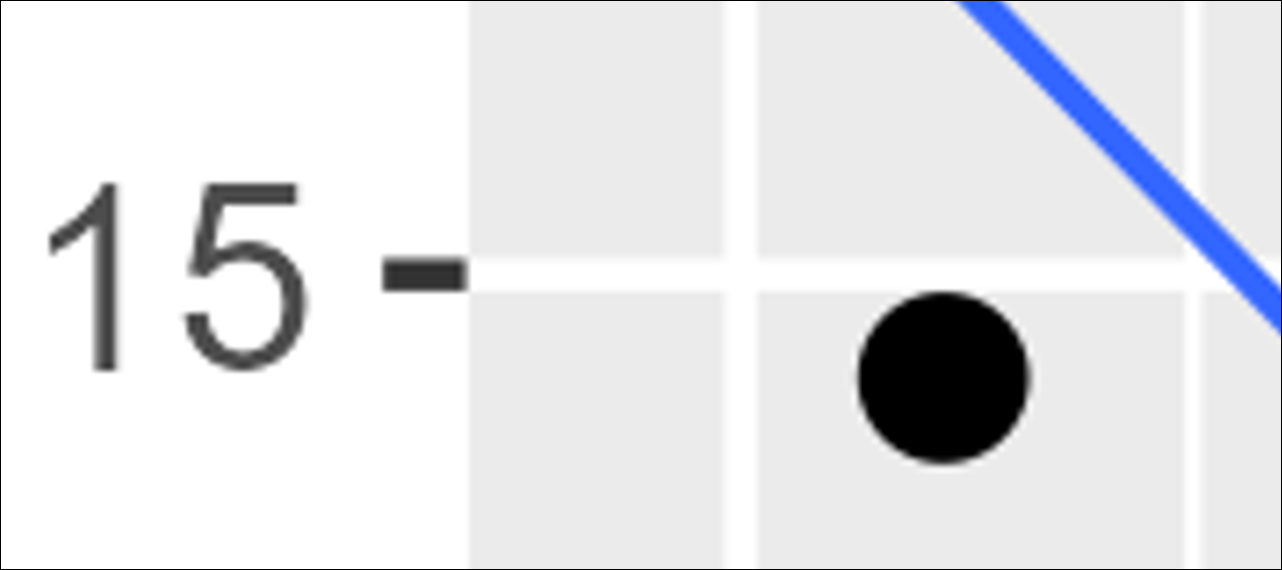
\includegraphics[scale = .3]{graphics/ch2Figs/artifacting_1.png}
\caption{Artificating present on our 300 dpi raster image when magnified.}
\end{figure}

A close inspection reveals jaggedness on the blue line and general blurriness around the rest of the image's elements. In academic publications, manuscripts, and presentations, this is something you want to avoid because, while these problems may not be immediately noticeable at first glance, they can impact a person's sensation of the image and, by extension, their opinion of its creator. Moreover, imperfections like these can be exacerbated in the printing and publishing process.

Now you might think that a simple remedy would be to increase the dpi to a much higher value, but this is generally a strategy you want to avoid.  There tends to be diminishing returns with resolution increases and anything beyond 300 dpi is not going to do much for you apart from ballooning the image's file size. The optimal strategy is to make use of something called a vector graphic.

Vector graphics are not really images in the traditional sense; rather, they are more akin to a set of instructions your computer uses to draw the image. Consequently, a vector-based image can be resized and magnified as much as you would like and it will never lose its quality. The drawback to vector graphics is that they do not work too well for highly detailed photographs (e.g., a forested landscape) and they are not always recognized by software. For instance, the most common types of vector you will encounter are .PDF, .SVG, and .EPS.  Recent versions of Microsoft Word and PowerPoint will happily accommodate .SVG files, but if you are wanting to use a .PDF or .EPS, you will be out of luck. Correspondingly, Google Docs and Google Slides will not accept any type of vector graphic, which is doubly frustrating because these apps will also downscale the resolution of raster graphics you import. Libre Office's Writer and Impress applications will accept a .PDF image, but it converts it to a lower resolution raster graphic when it is imported. Despite these types of compatibility limitations, if you are able to use vector graphics then you should, because they will give your work a level polish other people are not likely to have.

To save a file as a vector graphic, the process is the same as before, we just need to modify the file extension and remove the \R{dpi} argument (because dpi has no meaning for vector graphics).

\begin{inR}
ggsave("msleep_plot.svg", units = "cm", width = 20, height = 7)
\end{inR}

\vspace{1em}

The above code saved the image as a .SVG (Scalable Vector Graphic) file. This is a commonly used image file in web design, meaning it will, by default, be most likely displayed within a web-browser when you open it.

\begin{figure}[H]
\centering
\includesvg[scale = .3]{graphics/ch2Figs/artifacting_2.svg}
\caption{Magnification of a vector graphic.}
\end{figure}


\section{Scales}

A core concept in the ``grammar'' of \textit{ggplot2} is that of scales. Scales control how data is mapped to different aesthetics. For instance, there are scales for position, colour, size, shape, linetype, and so on. When you map an aesthetic to a variable like we did above where we had mapped both colour and shape to the \R{\$vore} column - e.g.,

\begin{inR}
...
geom_point(aes(colour = vore, shape = vore))
...
\end{inR}

\vspace{2em}

\begin{figure}[H]
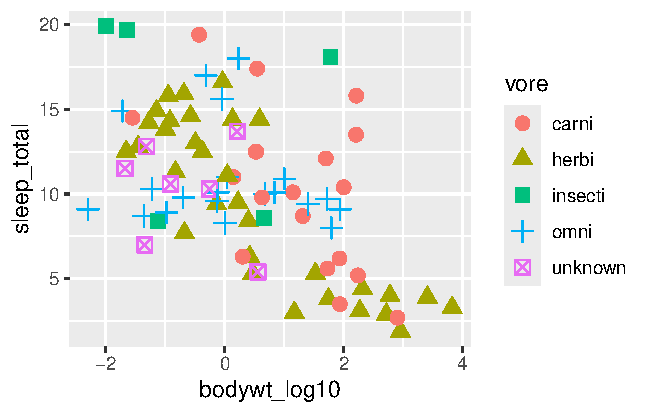
\includegraphics[scale = 0.75]{graphics/ch2Figs/ggEx_9.pdf}
\end{figure}

\vspace{1em}

\noindent
\textit{ggplot2} automatically chose which colours and shapes got applied to each category, but you can use functions to override these automatic mappings. 

The function you use to make these overrides is going to be dictated by the aesthetic you want to modify. For instance, to adjust the colour (or edge colour) of a point you could use \R{scale\_\textbf{colour}\_discrete()} function or the \R{scale\_\textbf{colour}\_continuous()} function. If you wanted to adjust the shapes of the points, you could use \R{scale\_\textbf{shape}\_discrete()} function.  If you wanted to adjust the fill colour of something (e.g., the fill colour of points or the fill colour of bars on a graph), you could use \R{scale\_\textbf{fill}\_discrete()} function or the \R{scale\_\textbf{fill}\_continuous()} function.

There are a large amount of functions like these and, at this point, you do not need to concern yourself with all their varieties and how they work. What is important to recognize here is that each scale function specifies, inside its name, what aesthetic (e.g., colour, shape, fill, etc.) it is modifying:

\begin{center}
    \R{scale\_\textit{<aesthetic name>}\_\textit{<transformation>}()}
\end{center}

The ``transformation'' part of the function's name is intended to describe how the function modifies the aesthetic which will hopefully become more apparent as we move through some examples.

\subsection{Position Scales: Modifying the Axis Breaks}
\label{sec:pos_scale}

When we first created the grid on to which we drew our points, we had actually mapped some aesthetics to do this. Specifically, we mapped the x and y aesthetics to the \R{\$bodywt} and \R{\$sleep\_total} columns respectively. In other words, we had written:

\begin{inR}
ggplot(data = msleep, aes(x = bodywt, y = sleep_total))
\end{inR}

\vspace{1em}

When first mapping the x and y axes of a plot, \textit{ggplot2} typically selects an appropriate sequence of values to display for each. These are what are referred to as axis \textit{breaks} and, most of the time, \textit{ggplot2}'s default scaling for the breaks is excellent. However, there are occasions where more customized scaling is necessary. In these situations, the following four functions are useful:

\begin{enumerate}
\setlength\itemsep{-1em}
    \item \R{scale\_x\_continuous()}
    \item \R{scale\_y\_continuous()}
    \item \R{scale\_x\_discrete()}
    \item \R{scale\_y\_discrete()}
\end{enumerate}

\noindent
The above four functions allow you to easily modify what values appear on your axis; though, which one you use depends on whether your axis has a \textit{continuous} or \textit{discrete} \gls{position scale}. Position scales control the location mappings of a plots visual elements.

In the case of the mammal sleep data we plotted, both the x-axis scale (body weight) and y-axis scale (sleep total) are \textit{continuous} in nature. In other words, the axis values represent measured numeric values as opposed to categories. Another way of conceptualizing this continuous vs discrete distinction is to approach it from R's perspective. In this case, both axes represent \textit{numeric} objects as opposed to \textit{character} objects. Thus, for the purpose of plotting, they are treated as a continuous scale.

\begin{inR}
mode(msleep$bodywt_log10) # x-axis
mode(msleep$sleep_total) # y-axis
\end{inR}
\begin{outR}
[1] "numeric"
[1] "numeric"
\end{outR}

If we had, for instance, plotted a categorical variable on the x-axis (e.g., the conservation status of the animal) then the x-axis would be discrete while the y-axis remains continuous (we will see an example of this later on).

To customize the breaks on our axis, we simply need to add one of the aforementioned functions to our plot's code and provide a vector of values we want to see displayed using the argument \R{breaks}. For instance, if we want the x-axis to only display the numbers 1, 2, and 3, we would add \\ \R{scale\_x\_continuous(breaks = c(1,2,3))} to our code (see line 11).

\begin{inR}
ggplot(msleep, aes(x = bodywt_log10, y = sleep_total)) +
  geom_point(size = 3) +
  geom_smooth(
    method = "lm",
    se = FALSE,
    linewidth = 0.5
  ) +
  facet_wrap(~vore, nrow = 1) +
  xlab("Log10(Body Weight kg)") + 
  ylab("Sleep Total (hrs)") + 
  scale_x_continuous(breaks = c(1,2,3))
\end{inR}

\vspace{2em}

\begin{figure}[H]
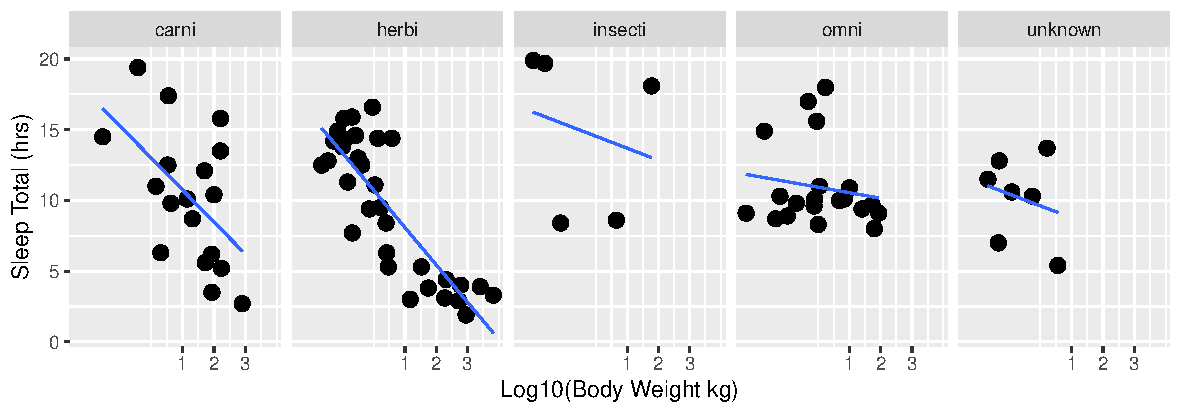
\includegraphics[scale = .75]{graphics/ch2Figs/ggEx_17.pdf}
\end{figure}

In general, the best practice is not to specify values individually, but rather specify a sequence using the \R{seq()} function we learned about in Chapter 1 (see section \ref{sec:func_args}). For instance, we could have the x-axis increment by 1s and the y-axis increment by 2s (see lines 11 and 12).

\begin{inR}
ggplot(msleep, aes(x = bodywt_log10, y = sleep_total)) +
  geom_point(size = 3) +
  geom_smooth(
    method = "lm",
    se = FALSE,
    linewidth = 0.5
  ) +
  facet_wrap(~vore, nrow = 1) +
  xlab("Log10(Body Weight kg)") + 
  ylab("Sleep Total (hrs)") + 
  scale_x_continuous(breaks = seq(-2, 4, 1)) +
  scale_y_continuous(breaks = seq(0, 20, 2))
\end{inR}

\vspace{2em}

\begin{figure}[H]
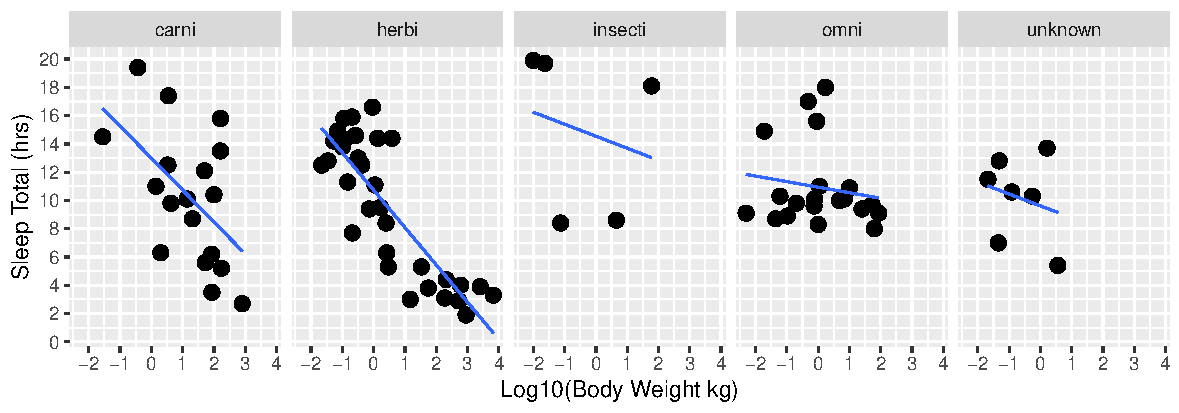
\includegraphics[scale = .75]{graphics/ch2Figs/ggEx_18.pdf}
\end{figure}

The four scale functions above can achieve a lot more than what is being shown here, but for most uses, this basic adjustment of the axis breaks will be their primary purpose.

\subsection{Modifying the Axis Range}

In addition to axis break adjustment, the range of the axis will often require customization as well.  To achieve this, the best practice is usually to use the function \R{coord\_cartesian()}.  To illustrate with some absurd values, we could have the x-axis span between -2 and +1 and have the y-axis span between $-5$ and $+10$.

\begin{inR}
ggplot(msleep, aes(x = bodywt_log10, y = sleep_total)) +
  geom_point(size = 3) +
  geom_smooth(
    method = "lm",
    se = FALSE,
    linewidth = 0.5
  ) +
  facet_wrap(~vore, nrow = 1) +
  xlab("Log10(Body Weight kg)") + 
  ylab("Sleep Total (hrs)") +
  scale_x_continuous(breaks = seq(-2, 4, 1)) +
  scale_y_continuous(breaks = seq(0, 20, 2)) +
  coord_cartesian(xlim = c(-2, 1), ylim = c(-5, 10))
\end{inR}

\vspace{2em}

\begin{figure}[H]
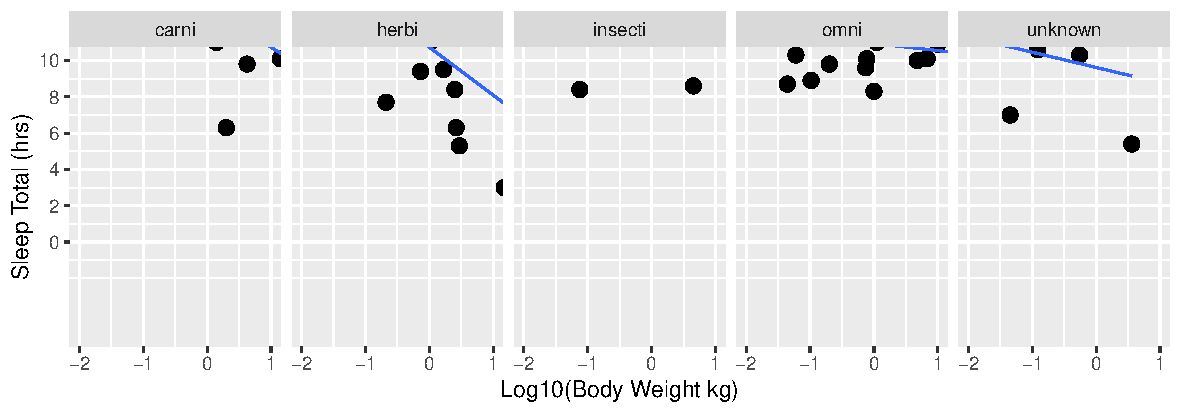
\includegraphics[scale = .75]{graphics/ch2Figs/ggEx_19.pdf}
\end{figure}

\noindent
Note that, while the y-axis goes as low as -5, it does not show breaks below 0 because of how the \R{breaks} argument in \R{scale\_y\_continuous()} were set.

At this point it is worth offering a disclaimer.  Within the position scale functions mentioned earlier (i.e., \R{scale\_x\_continuous()} and \R{scale\_y\_continuous()}, there is an argument called \R{limits} that will allow you to set the range of the scale in a manner similar to the \R{coord\_cartesian()} function. Additionally, \textit{ggplot2} also has two other functions, \R{xlim()} and \R{ylim()}, that will do the same. However, setting the limits of your plot with these arguments and functions is best avoided because they will remove data falling outside of those specified limits. This can result in problems if your plot's code is performing some type of statistical calculation. For instance, if you remove lines 12 and 13 in the above script and add \R{ylim(-2, 1)} you will be confronted with a very nasty error message, telling you (among other things) that ...

\begin{outR}
Warning messages:
1: Removed 83 rows containing non-finite outside the scale range
(`stat_smooth()`). 
\end{outR}

\noindent
This occurs because values in our data falling outside of $-2$ and $+1$ are not recognized anymore, but \textit{ggplot2} needed those values to calculate that blue regression line using the \R{geom\_smooth()} function. Thus, the moral of the story is, if you need to ``zoom-in'' or ``zoom-out'' on a plot, use \R{coord\_cartesian()}. Do not be tempted by those other options.\footnote{Readers are probably wondering ``\textit{what use does removing data outside of the limits serve? It seems like it would only ever cause more problems than it solves (especially if you are unaware it is happening).}'' And to that I say, yes.}

\subsection{Colour Scales: Modifying Colour Mappings}

Similar to how \textit{ggplot2} automatically selected a scaling for the breaks on the x and y axis, it also automatically selected various colours to use when we mapped colour to the \R{$vore$} column. Moreover, the distinction between \textit{continuous} and \textit{discrete} scaling applies just as much to colour as it does position. As illustrated in Figure \ref{fig:continuous_col_scale} and \ref{fig:discrete_col_scale}, discrete colour scales are usually represented with a colour gradient and discrete scales are represented by distinct colours (like in a box of crayons). While it is possible to do this, you usually do not want to use a gradient to represent distinct categories because it makes the categories difficult to discriminate visually. For instance, the \R{\$vore} column we mapped to the colour aesthetic earlier contained distinct non-numeric categories (e.g., carni, herbi, insecti, and so on); thus, a colour palette such as that seen in Figure \ref{fig:discrete_col_scale} would be much more appropriate than Figure \ref{fig:continuous_col_scale}.

\vspace{2em}

\begin{figure}[h]
\centering

\includegraphics[scale = .4]{graphics/ch2Figs/col_gradient.pdf}
\caption{Example of a continuous colour scale (i.e., a colour gradient).}
\label{fig:continuous_col_scale}
\end{figure}

\vspace{2em}

\begin{figure}[H]
\centering

\includegraphics[scale = .4]{graphics/ch2Figs/col_discrete.pdf}
\caption{Example of a discrete colour scale (a.k.a. a qualitative palette.)}
\label{fig:discrete_col_scale}
\end{figure}

\vspace{1em}

\subsection{Discrete Colour Scales}
\label{sec:discrete_cols}

To illustrate the use of discrete colour scales lets create a simple plot we can experiment with.

\begin{inR}
ggplot(msleep, aes(x = bodywt_log10, y = sleep_total)) +
  geom_point(size = 3, shape = 21, stroke = 2)
\end{inR}

\vspace{2em}

\begin{figure}[H]
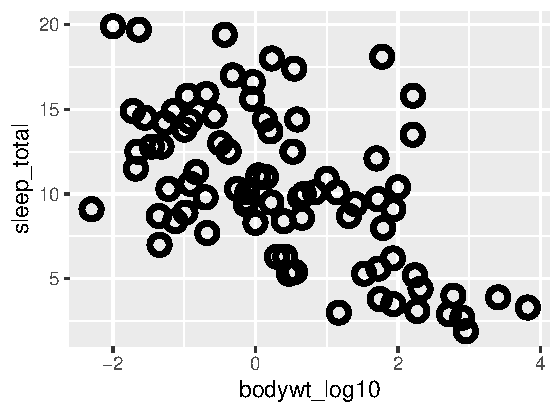
\includegraphics[scale = .75]{graphics/ch2Figs/ggEx_20.pdf}
\end{figure}

\noindent
First we will map the edge colour to the column \R{\$vore}.

\begin{inR}
ggplot(msleep, aes(x = bodywt_log10, y = sleep_total)) +
  geom_point(
    size = 3, shape = 21, stroke = 2,
    aes(colour = vore)
  )
\end{inR}

\vspace{2em}

\begin{figure}[H]
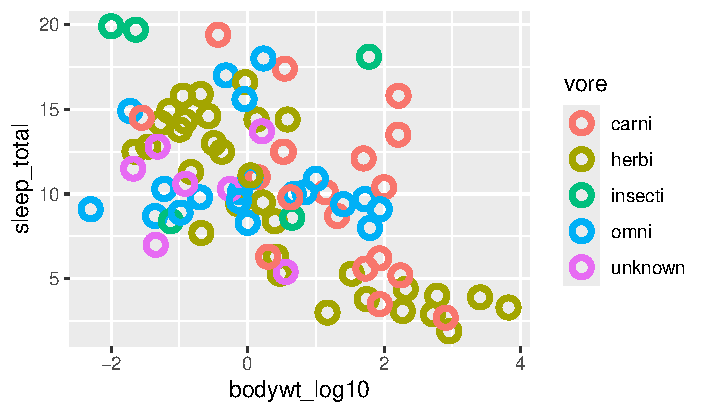
\includegraphics[scale = .75]{graphics/ch2Figs/ggEx_21.pdf}
\end{figure}

\noindent
Then, to override these colours we can simply use \R{scale\_colour\_discrete()} and input a vector of colours.

\begin{inR}
ggplot(msleep, aes(x = bodywt_log10, y = sleep_total)) +
  geom_point(
    size = 3, shape = 21, stroke = 2,
    aes(colour = vore)
  ) +
  scale_colour_discrete(type = c("red", "blue", "green", "purple", "orange"))
\end{inR}

\vspace{2em}

\begin{figure}[H]
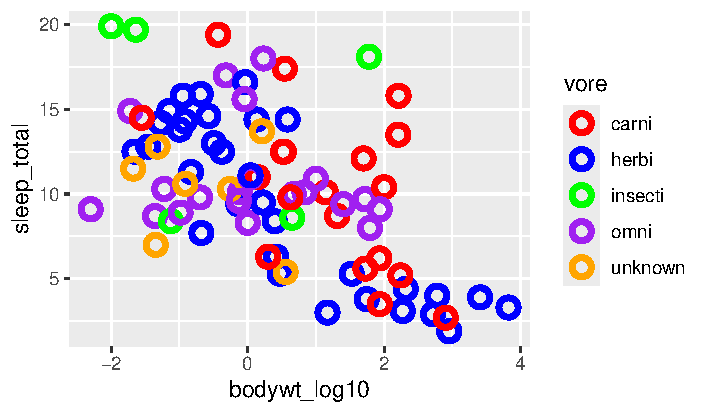
\includegraphics[scale = .75]{graphics/ch2Figs/ggEx_22.pdf}
\end{figure}

The same effect can be achieved by using \R{scale\_colour\_manual()} instead.

\begin{inR}
...
scale_colour_manual(values = c("red", "blue", "green", "purple", "orange"))
\end{inR}

\vspace{1em}

\noindent
However, the advantage to using \R{scale\_colour\_discrete()} is you are not limited by the number of categories in your palette. This means you can create a bigger colour palette and \textit{ggplot2} will only use as many colours as needed. By contrast, if you use \R{scale\_colour\_manual()}, you have to ensure that you specify the same amount of colours as there are categories. To illustrate, we can create a palette with eight colours, but \textit{ggplot2} will only use the first six.

\begin{inR}
# Create a colour palette
palette <- c(
  "#000000", "#DF536B", "#61D04F", "#2297E6", "#28E2E5", "#CD0BBC", "#F5C710",
  "#9E9E9E"
)

# Use that palette in your plot
ggplot(msleep, aes(x = bodywt_log10, y = sleep_total)) +
  geom_point(
    size = 3, shape = 21, stroke = 2,
    aes(colour = vore)
  ) +
  scale_colour_discrete(type = palette)
\end{inR}

\vspace{2em}

\begin{figure}[H]
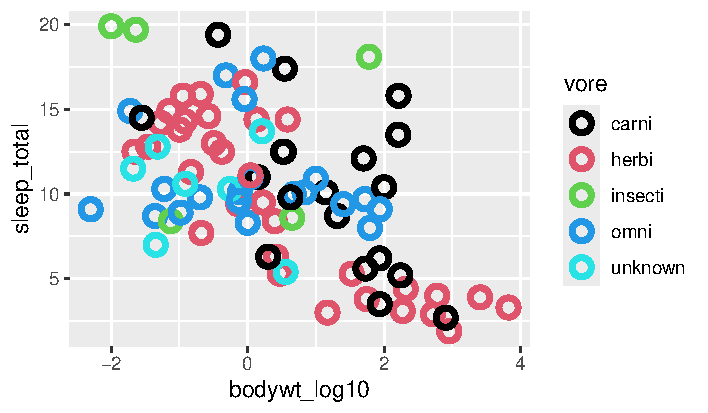
\includegraphics[scale = .75]{graphics/ch2Figs/ggEx_23.pdf}
\end{figure}


Notice that we are using pch 21 as our shape. Recall that this shape takes both an edge and fill colour (see Figure \ref{fig:points.pdf}). At present, we have not specified a fill colour, so the points are hollow. However, instead of modifying the edge colour like we have been doing, we could modify the fill colour of the points and just keep the edges black.

\begin{inR}
ggplot(msleep, aes(x = bodywt_log10, y = sleep_total)) +
  geom_point(
    size = 3, shape = 21, stroke = 1, colour = "black",
    aes(fill = vore)
  ) +
  scale_fill_discrete(type = palette)
\end{inR}

\vspace{2em}

\begin{figure}[H]
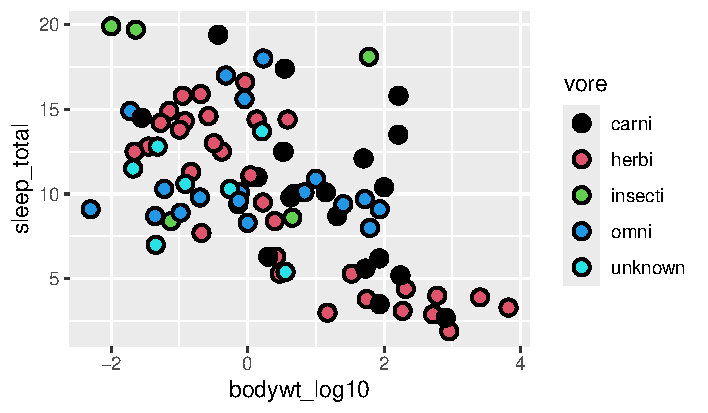
\includegraphics[scale = .75]{graphics/ch2Figs/ggEx_24.pdf}
\end{figure}

\noindent
Notice where the important changes have taken place in the code.  We have moved the \R{colour} aesthetic outside of the \R{aes()} function.  This means a single \R{colour} (black) will now be mapped to all the points. We have also mapped the \R{\$vore} column to the \R{fill} aesthetic inside of \R{aes()} and, for that reason, now specify \R{scale\_\textbf{fill}\_discrete()} to modify the colour options. In other words, we are now adjusting the \textit{fill} colour, not the point/edge colour.

\subsubsection{Pre-Existing Discrete Colour Palettes}

Until now, we have been specifying our own custom colour palettes; however, base R contains a variety of pre-existing palettes we can make use of. To obtain the list you can simply run the following:

\begin{inR}
palette.pals()
\end{inR}
\begin{outR}
 [1] "R3"              "R4"              "ggplot2"         "Okabe-Ito"      
 [5] "Accent"          "Dark 2"          "Paired"          "Pastel 1"       
 [9] "Pastel 2"        "Set 1"           "Set 2"           "Set 3"          
[13] "Tableau 10"      "Classic Tableau" "Polychrome 36"   "Alphabet"
\end{outR}

Of note, palettes \R{"R4"}, \R{"Okabe-Ito"}, \R{"Dark 2"}, \R{"Paired"}, and \R{"Set 2"}, are all decently robust under conditions of colour vision deficiency. To obtain a vector of the hex codes used for a specific palette, you can just run \R{palette.colors(n = NULL, "Dark 2")}, but it is usually more convenient to insert this function directly into \textit{ggplot2}. Figure \ref{fig:discrete_cols} illustrates the colours employed in each palette - only eight colours are shown but some do contain more.

\begin{inR}
ggplot(msleep, aes(x = bodywt_log10, y = sleep_total)) +
  geom_point(
    size = 3, shape = 21, stroke = 1, colour = "black",
    aes(fill = vore)
  ) +
  scale_fill_discrete(type = palette.colors(n = NULL, "Dark2"))
\end{inR}

\vspace{2em}

\begin{figure}[H]
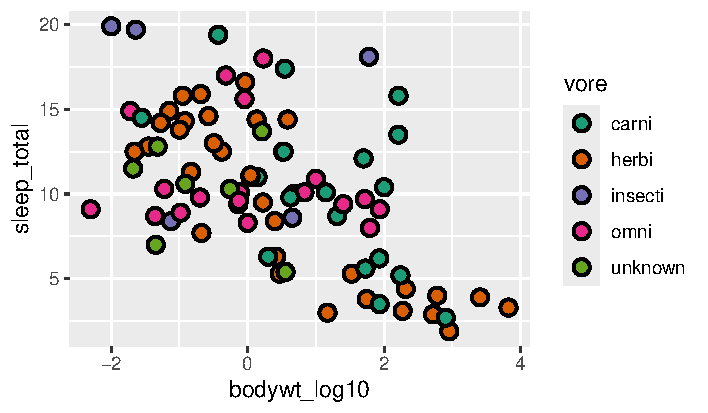
\includegraphics[scale = .75]{graphics/ch2Figs/ggEx_25.pdf}
\end{figure}

\vspace{2em}

\begin{figure}[h]
\centering
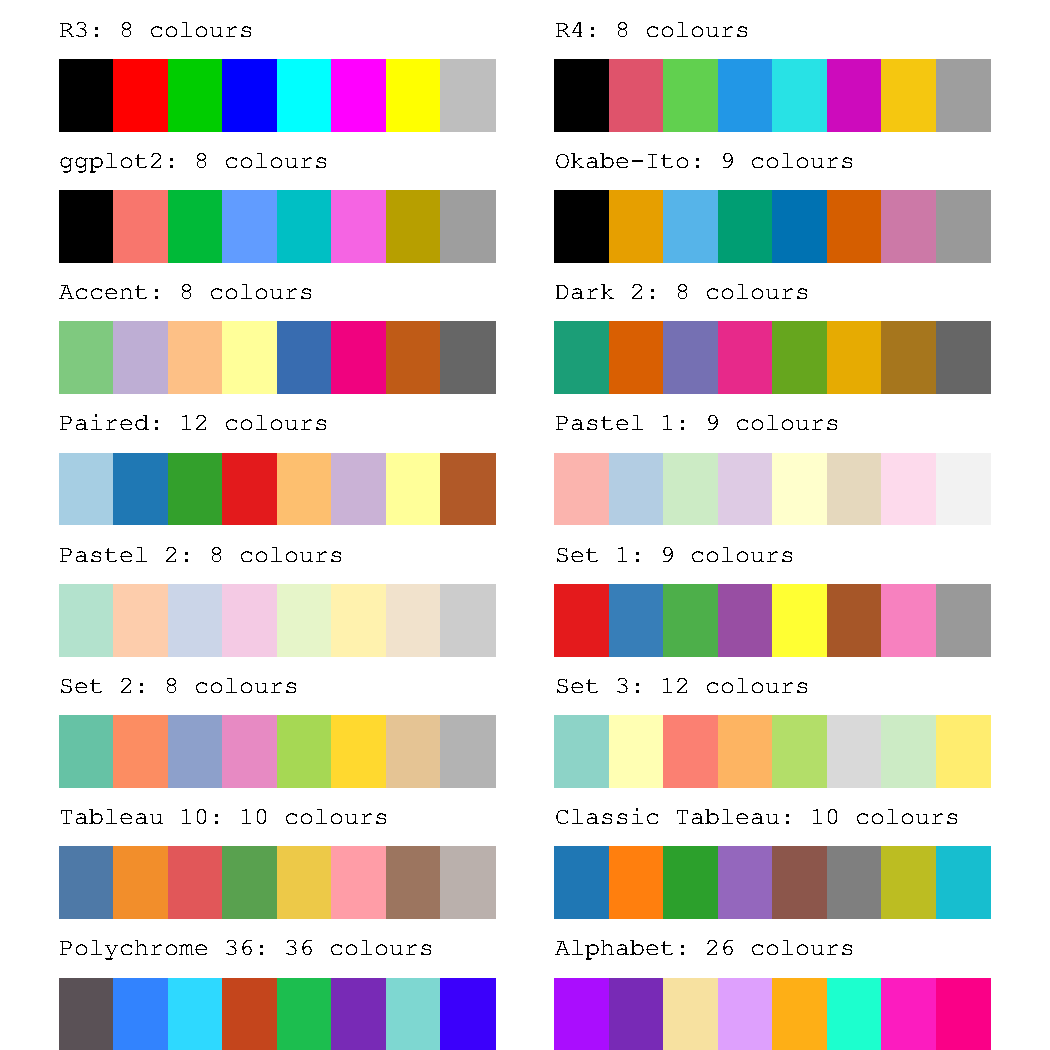
\includegraphics[scale = .6]{graphics/ch2Figs/palettes.pdf}
\caption{Examples of the various discrete colour palettes in base R.}
\label{fig:discrete_cols}
\end{figure}

\subsection{Continuous Colour Scales}

Continuous colour scales operate more or less in the same manner as discrete ones; however, to illustrate them, we need to map colour to a continuous variable. In the \R{msleep} data, there is a column called \R{\$brainwt} which, similar to \R{\$bodywt}, is a continuous measure. To visualize it adequately we will need to log transform it as well. For simplicity we will do this directly in the plot's code:

\begin{inR}
ggplot(msleep, aes(x = bodywt_log10, y = sleep_total)) +
  geom_point(
    size = 3, shape = 21, stroke = 1, colour = "black",
    aes(fill = log10(brainwt))
  )
\end{inR}

\vspace{2em}

\begin{figure}[H]
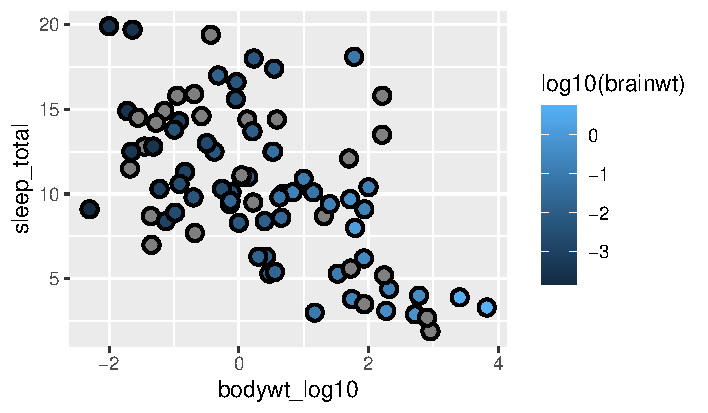
\includegraphics[scale = .75]{graphics/ch2Figs/ggEx_26.pdf}
\end{figure}

Immediately you can see we are now presented with a \textit{colourbar} instead of a set of fixed colours. This is because the nature of the variable \R{\$brainwt} is that it is continuous. Thus, it does not fall neatly into distinct categories.  Between any two brain weights there is a theoretically infinite amount of values and the colourbar's gradient offers a means of representing that. As you move from black to blue, lighter shades of blue are indicative of a heavier brain weight. Looking at the graph, increases in body weight also seem to correspond to increases in brain weight, but notice the grey points in the graph.  Those are indicative of missing values in the \R{\$brainwt} column and with a bit of R code, we can filter the data to see what values these are specifically.

\begin{inR}
filter(msleep, is.na(brainwt))
\end{inR}

\vspace{1em}

In case it is not obvious, this code works by using the \R{is.na()} function to check whether each row in the \R{msleep} data frame's  \R{\$brainwt} column contains an \R{NA} value. Rows which result as \R{TRUE} are displayed and everything else is ignored. This leaves us with a data frame of 27 different animals, all of which have a \R{NA} value in the \R{\$brainwt} column.


If you are left unsatisfied by the default black to blue gradient, \textit{ggplot2} makes it easy to produce custom colour gradients using the \R{scale\_fill\_gradient()} and \R{scale\_fill\_gradient2()} functions, and of course there are colour aesthetic variants of this for situations where you want to modify the edge and point colours.\footnote{These are \R{scale\_colour\_gradient()} and \R{scale\_colour\_gradient2()}.} Both functions simply require you to specify a \R{low} colour argument that represents the bottom of the colourbar and a \R{high} colour argument that represents the top of the colour bar. However, \R{scale\_colour\_gradient2()} also requires you to specify the argument \R{mid}, which indicates a third midpoint colour. You can even specify the location of this midpoint with the argument \R{midpoint}. More succinctly \R{scale\_colour\_gradient()} creates \textit{sequential} colour palettes, and \R{scale\_colour\_gradient2()} creates \textit{diverging} colour palettes.

In addition to those main arguments, you can also specify what colour you would like \R{NA} values to be represented by and set the the breaks that appear on the colourbar. These are given by the arguments \R{na.value} and \R{breaks} respectively.

\begin{inR}
# scale_colour_gradient example
ggplot(msleep, aes(x = bodywt_log10, y = sleep_total)) +
  geom_point(
    size = 3, shape = 21, stroke = 1, colour = "black",
    aes(fill = log10(brainwt))
  ) +
  scale_fill_gradient(
    low = "blue",
    high = "red",
    na.value = "green", 
    breaks = seq(-4, 1, 1)
  )
\end{inR}

\vspace{2em}

\begin{figure}[H]
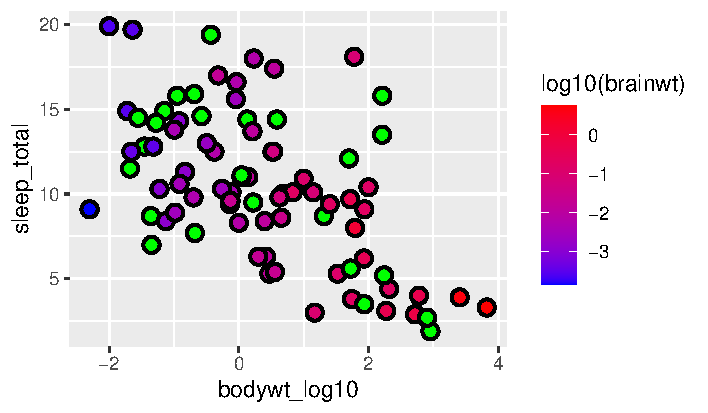
\includegraphics[scale = .75]{graphics/ch2Figs/ggEx_27.pdf}
\end{figure}

With the mammal sleep data, there is no logical reason to plot a midpoint colour using \\ \R{scale\_colour\_gradient2()} but to illustrate its use we will depict a midpoint using the colour \R{"grey"} and we will place it at a $\text{log}_{10}(\text{brain weight}) = -1.5$.

\begin{inR}
# scale_colour_gradient2 example
ggplot(msleep, aes(x = bodywt_log10, y = sleep_total)) +
  geom_point(
    size = 3, shape = 21, stroke = 1, colour = "black",
    aes(fill = log10(brainwt))
  ) +
  scale_fill_gradient2(
    low = "blue",
    mid = "grey",
    high = "red",
    midpoint = -1.5,
    na.value = "green", 
    breaks = seq(-4, 1, 1)
  )
\end{inR}

\vspace{2em}

\begin{figure}[H]
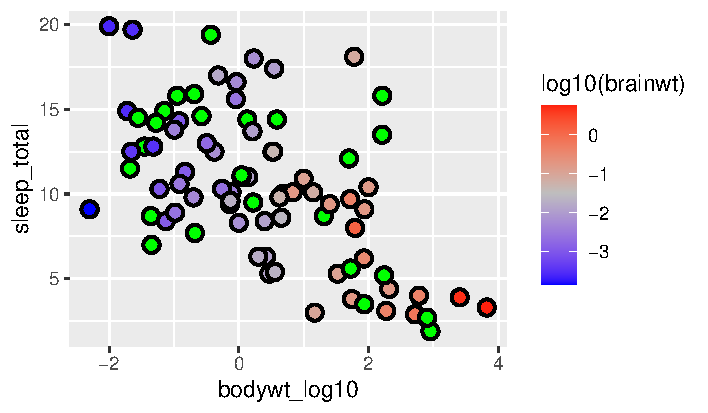
\includegraphics[scale = .75]{graphics/ch2Figs/ggEx_28.pdf}
\end{figure}

\subsubsection{Pre-Existing Continuous Colour Palettes}

Similar to what we saw with discrete colour scales, R comes with a set of continuous colour palettes we can use, some of which are sequential and some of which are diverging. For those interested, these palettes are based around an HCL (hue-chroma-luminance) colour space model which confers some advantages over the HSV (hue-saturation-value) colour space model computers have traditionally employed \parencite{Zeileis2019}.

To obtain a list of these HCL palettes you can simply run any of the following lines for sequential, diverging, and qualitative palettes respectively.

\begin{inR}
hcl.pals(type = "sequential")
hcl.pals(type = "diverging")
hcl.pals(type = "qualitative")
\end{inR}

\vspace{1em}

The qualitative palettes work best for discrete scales (i.e., identifying distinct categories) where you want each category to have equal perceptual weight. These are not much use for our present purposes but are notable because they are based on a HCL colour space model. That means we are not limited by the amount of colours in the palette like we were with R's standard discrete colour palettes (see section \ref{sec:discrete_cols}). Though, anecdotally, when you go beyond 6 categories the HCL qualitative palettes' colours start to become more and more difficult to discriminate between (even with standard colour vision). Interestingly, \textit{ggplot2}'s default discrete colour selection relies on a similar underlying theory.

To obtain the hex codes for any given palette (e.g., \R{"Inferno"}) you will, in addition to providing the palette name, need to specify how many hex codes you want to see using the argument \R{n}. Visual examples of the three HCL palette types are provided in Appendix \ref{sec:AppendixPalettes}.

\begin{inR}
hcl.colors(n = 8, palette = "Inferno") 
\end{inR}
\begin{outR}
[1] "#040404" "#341348" "#701069" "#AB1E75" "#DC4962" "#F58426" "#F8C149" "#FFFE9E"
\end{outR}

To use one of base R's HCL colour palettes in our plot we can use the function \\ \R{scale\_fill\_gradientn()} to set our palette. The function just takes a vector of colours and extrapolates a gradient from that.

\begin{inR}
ggplot(msleep, aes(x = bodywt_log10, y = sleep_total)) +
  geom_point(
    size = 3, shape = 21, stroke = 1, colour = "black",
    aes(fill = log10(brainwt))
  ) +
  scale_fill_gradientn(
    colours = hcl.colors(n = 50, palette = "Inferno"),
    na.value = "grey", 
    breaks = seq(-4, 1, 1)
  )
\end{inR}

\vspace{2em}

\begin{figure}[H]
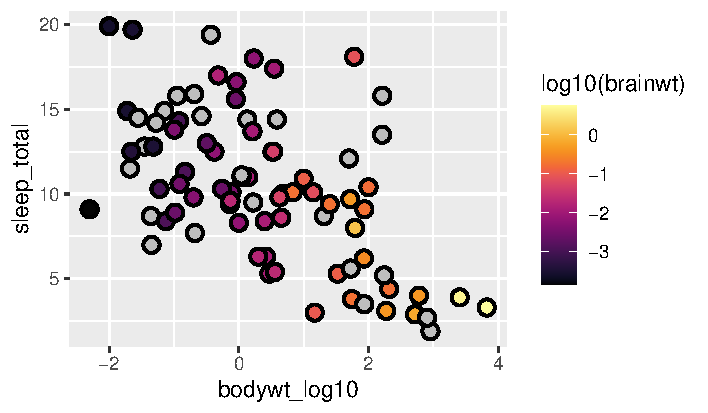
\includegraphics[scale = .75]{graphics/ch2Figs/ggEx_29.pdf}
\end{figure}

\subsection{Shape Scales}

We know that relying solely on colour to visually discriminate categories is inadvisable due to colour vision deficiencies people may have; thus, in addition to adjusting the colour scales, we can also adjust the shape scale simultaneously by mapping \R{\$vore} to both \R{shape} and \R{fill} within the \R{aes()} function. For the shapes we will use the pch symbols 21 - 24 and also have the category ``unknown'' be represented by pch 13 (see Figure \ref{fig:points.pdf}) - recall that these particular symbols (21 - 24) take both a colour and fill aesthetic. We will keep the edges (i.e., colour aesthetic) black but, for the fill aesthetic, we will use the \R{"R4"} colour palette (see Figure \ref{fig:discrete_cols}).

\begin{inR}
ggplot(msleep, aes(x = bodywt_log10, y = sleep_total)) +
  geom_point(
    size = 3, stroke = 1, colour = "black",
    aes(fill = vore, shape = vore)
  ) +
  scale_shape_manual(values = c(21:24), na.value = 13) +
  scale_fill_discrete(type = palette.colors(n = NULL, "R4"))
\end{inR}

\vspace{2em}

\begin{figure}[H]
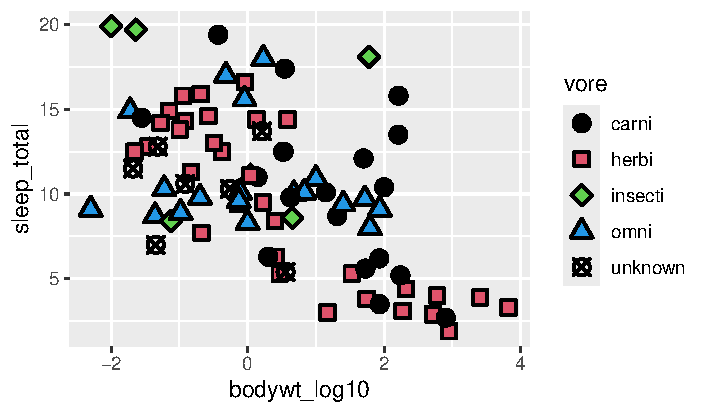
\includegraphics[scale = .75]{graphics/ch2Figs/ggEx_30.pdf}
\end{figure}

\subsection{Legend Titles}

In all the examples above, the legend that \textit{ggplot2} produced has always been titled with the name of the column it is representing. For instance, when we mapped the categories in the \R{\$vore} column it was titled ``vore.'' When we mapped \R{log10(brainwt}, it was titled ``log10(brainwt).'' To adjust the name of the legend, each \R{scale} function we have used also takes a \R{name} argument which will dictate how the legend is titled. For instance, keeping with the above example, we could adjust the legend title to read "Diet".

\begin{inR}
ggplot(msleep, aes(x = bodywt_log10, y = sleep_total)) +
  geom_point(
    size = 3, stroke = 1, colour = "black",
    aes(fill = vore, shape = vore)
  ) +
  scale_shape_manual(values = c(21:24), na.value = 13, name = "Diet") +
  scale_fill_discrete(type = palette.colors(n = NULL, "R4"), name = "Diet")
\end{inR}

\vspace{2em}

\begin{figure}[H]
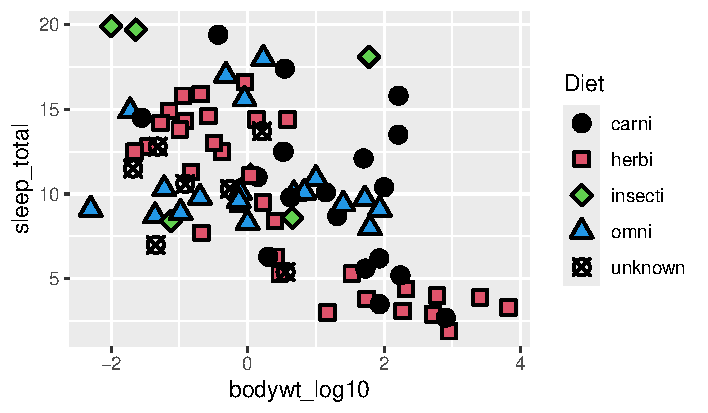
\includegraphics[scale = .75]{graphics/ch2Figs/ggEx_31.pdf}
\end{figure}

In this example, we have two scales in our legend, the \R{shape} scale and the \R{fill} scale.  If you do not specify an identical name for each, they will be treated as separate legends. For instance, try giving \R{scale\_shape\_manual()} a different name than \R{scale\_fill\_discrete()} and see what happens.

An alternative method for renaming your legend is to add the function \R{labs()} to your plot's code and specify the name of each scale as a separate argument.

\begin{inR}
ggplot(msleep, aes(x = bodywt_log10, y = sleep_total)) +
  geom_point(
    size = 3, stroke = 1, colour = "black",
    aes(fill = vore, shape = vore)
  ) +
  scale_shape_manual(values = c(21:24), na.value = 13) +
  scale_fill_discrete(type = palette.colors(n = NULL, "R4")) +
  labs(
    shape = "Diet",
    fill = "Diet"
  )
\end{inR}

\vspace{1em}

\subsection{Other Scales}

In the sections above, we have only considered the position, colour, fill, and shape scales, which are among the features most frequently appealed to when graphing, but similar functions exist for other scales. For instance, there are scale functions to modify the size, linewidth, and linetype aesthetics if needed. To learn more about these and other features, an excellent resource is the tidyverse's official \textit{ggplot2} website, which contains a learning section that will direct you to various excellent resources (\url{https://ggplot2.tidyverse.org/}), the best and most comprehensive of which is the official manual for \textit{ggplot2} titled ``ggplot2: Elegant Graphics for Data Analysis.'' Keeping with the ethos of ``free software'', this is available to read online for free at 

\begin{center}
\url{https://ggplot2-book.org/}
\end{center}

\section{Modifying Other Non-data Components}

One thing that will be apparent is that \textit{ggplot2} has a very specific ``look'' to it, and that look is not arbitrary. It was crafted meticulously on the basis of expert advice. In the language of \textit{ggplot2}, this look is what is referred to as a \textit{theme}.  Specifically, we are seeing \R{theme\_grey()} and in the dark master's own words:

\begin{displayquote}
\headingfont
%\large
The theme is designed to put the data forward while supporting comparisons, following the advice of Tufte \citeyear{Tufte2006}; Brewer \citeyear{Brewer1994}; Carr \citeyear{Carr2002}, \citeyear{Carr1994}; Carr and Sun \citeyear{Carr1999}. We can still see the gridlines to aid in the judgement of position \parencite{Cleveland1993}, but they have little visual impact and we can easily `tune' them out. The grey background gives the plot a similar typographic colour to the text, ensuring that the graphics fit in with the flow of a document without jumping out with a bright white background. Finally, the grey background creates a continuous field of colour which ensures that the plot is perceived as a single visual entity.

- \cite{Wickham_ggplot2}

\end{displayquote}

\noindent
To sum up, the grey theme is immaculate in its conception and cannot be improved upon. In fact, once one has borne witness to the majesty of \R{theme\_grey()}, even small departures from it can have drastic effects on a person's physical and mental well being. That being said, \textit{ggplot2} still offers its users the ability to modify any aspect of the plot they wish - just be careful what you wish for.

\subsection{Built-in Themes}

Once the scaling and other main visual elements related to data presentation are complete, it is often helpful to set your plot's code as a variable you can append other elements to. Meaning that, in the same way a number in R is an object that you can name and add things to - e.g., 

\begin{inR}
x <- 1
x + 2
\end{inR}
\begin{outR}
[1] 3
\end{outR}

\noindent
your plot is also an object (just a very complex one) that you can \textit{add} things to. For instance, on the first line of our plot's code, right before the function \R{ggplot()}, we could give our plot the name \R{my\_plot}.

\begin{inR}
my_plot <- ggplot(msleep, aes(x = bodywt_log10, y = sleep_total)) +
  geom_point(
    size = 3, colour = "black",
    aes(fill = vore, shape = vore)
  ) +
  scale_shape_manual(values = c(21:24, 13)) +
  scale_fill_discrete(type = palette.colors(n = NULL, "R4")) +
  labs(
    shape = "Diet",
    fill = "Diet"
  ) +
  xlab("Log10(Body Weight kg)") + ylab("Sleep Total (hrs)")
\end{inR}

\vspace{1em}

\noindent
Now, when you run \R{my\_plot} you can see it output to the plot window.

\begin{inR}
my_plot 
\end{inR}

\vspace{2em}

\begin{figure}[H]
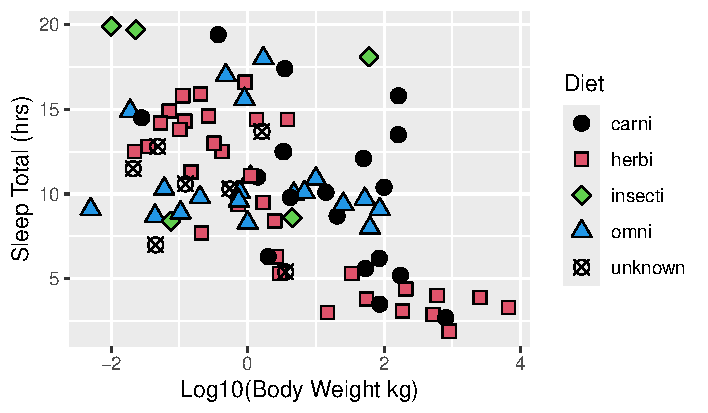
\includegraphics[scale = .75]{graphics/ch2Figs/ggEx_32.pdf}
\end{figure}

The quickest way to modify the overall appearance of your plot - which works well as a starting point for other modifications you want to make - is to use one of ggplot2's built in themes shown in Figure \ref{fig:gg_built-in-themes}.  Simply add the theme's function to your plot's code.  For instance, if you wanted to use the black and white theme, \R{theme\_bw()}, you would run ...

\begin{inR}
my_plot + theme_bw()
\end{inR}

\vspace{1em}

\noindent
Additional pre-built themes can be accessed via other R packages, such as \R{ggthemes}.

\vspace{2em}

\begin{figure}[h]
\centering
\frame{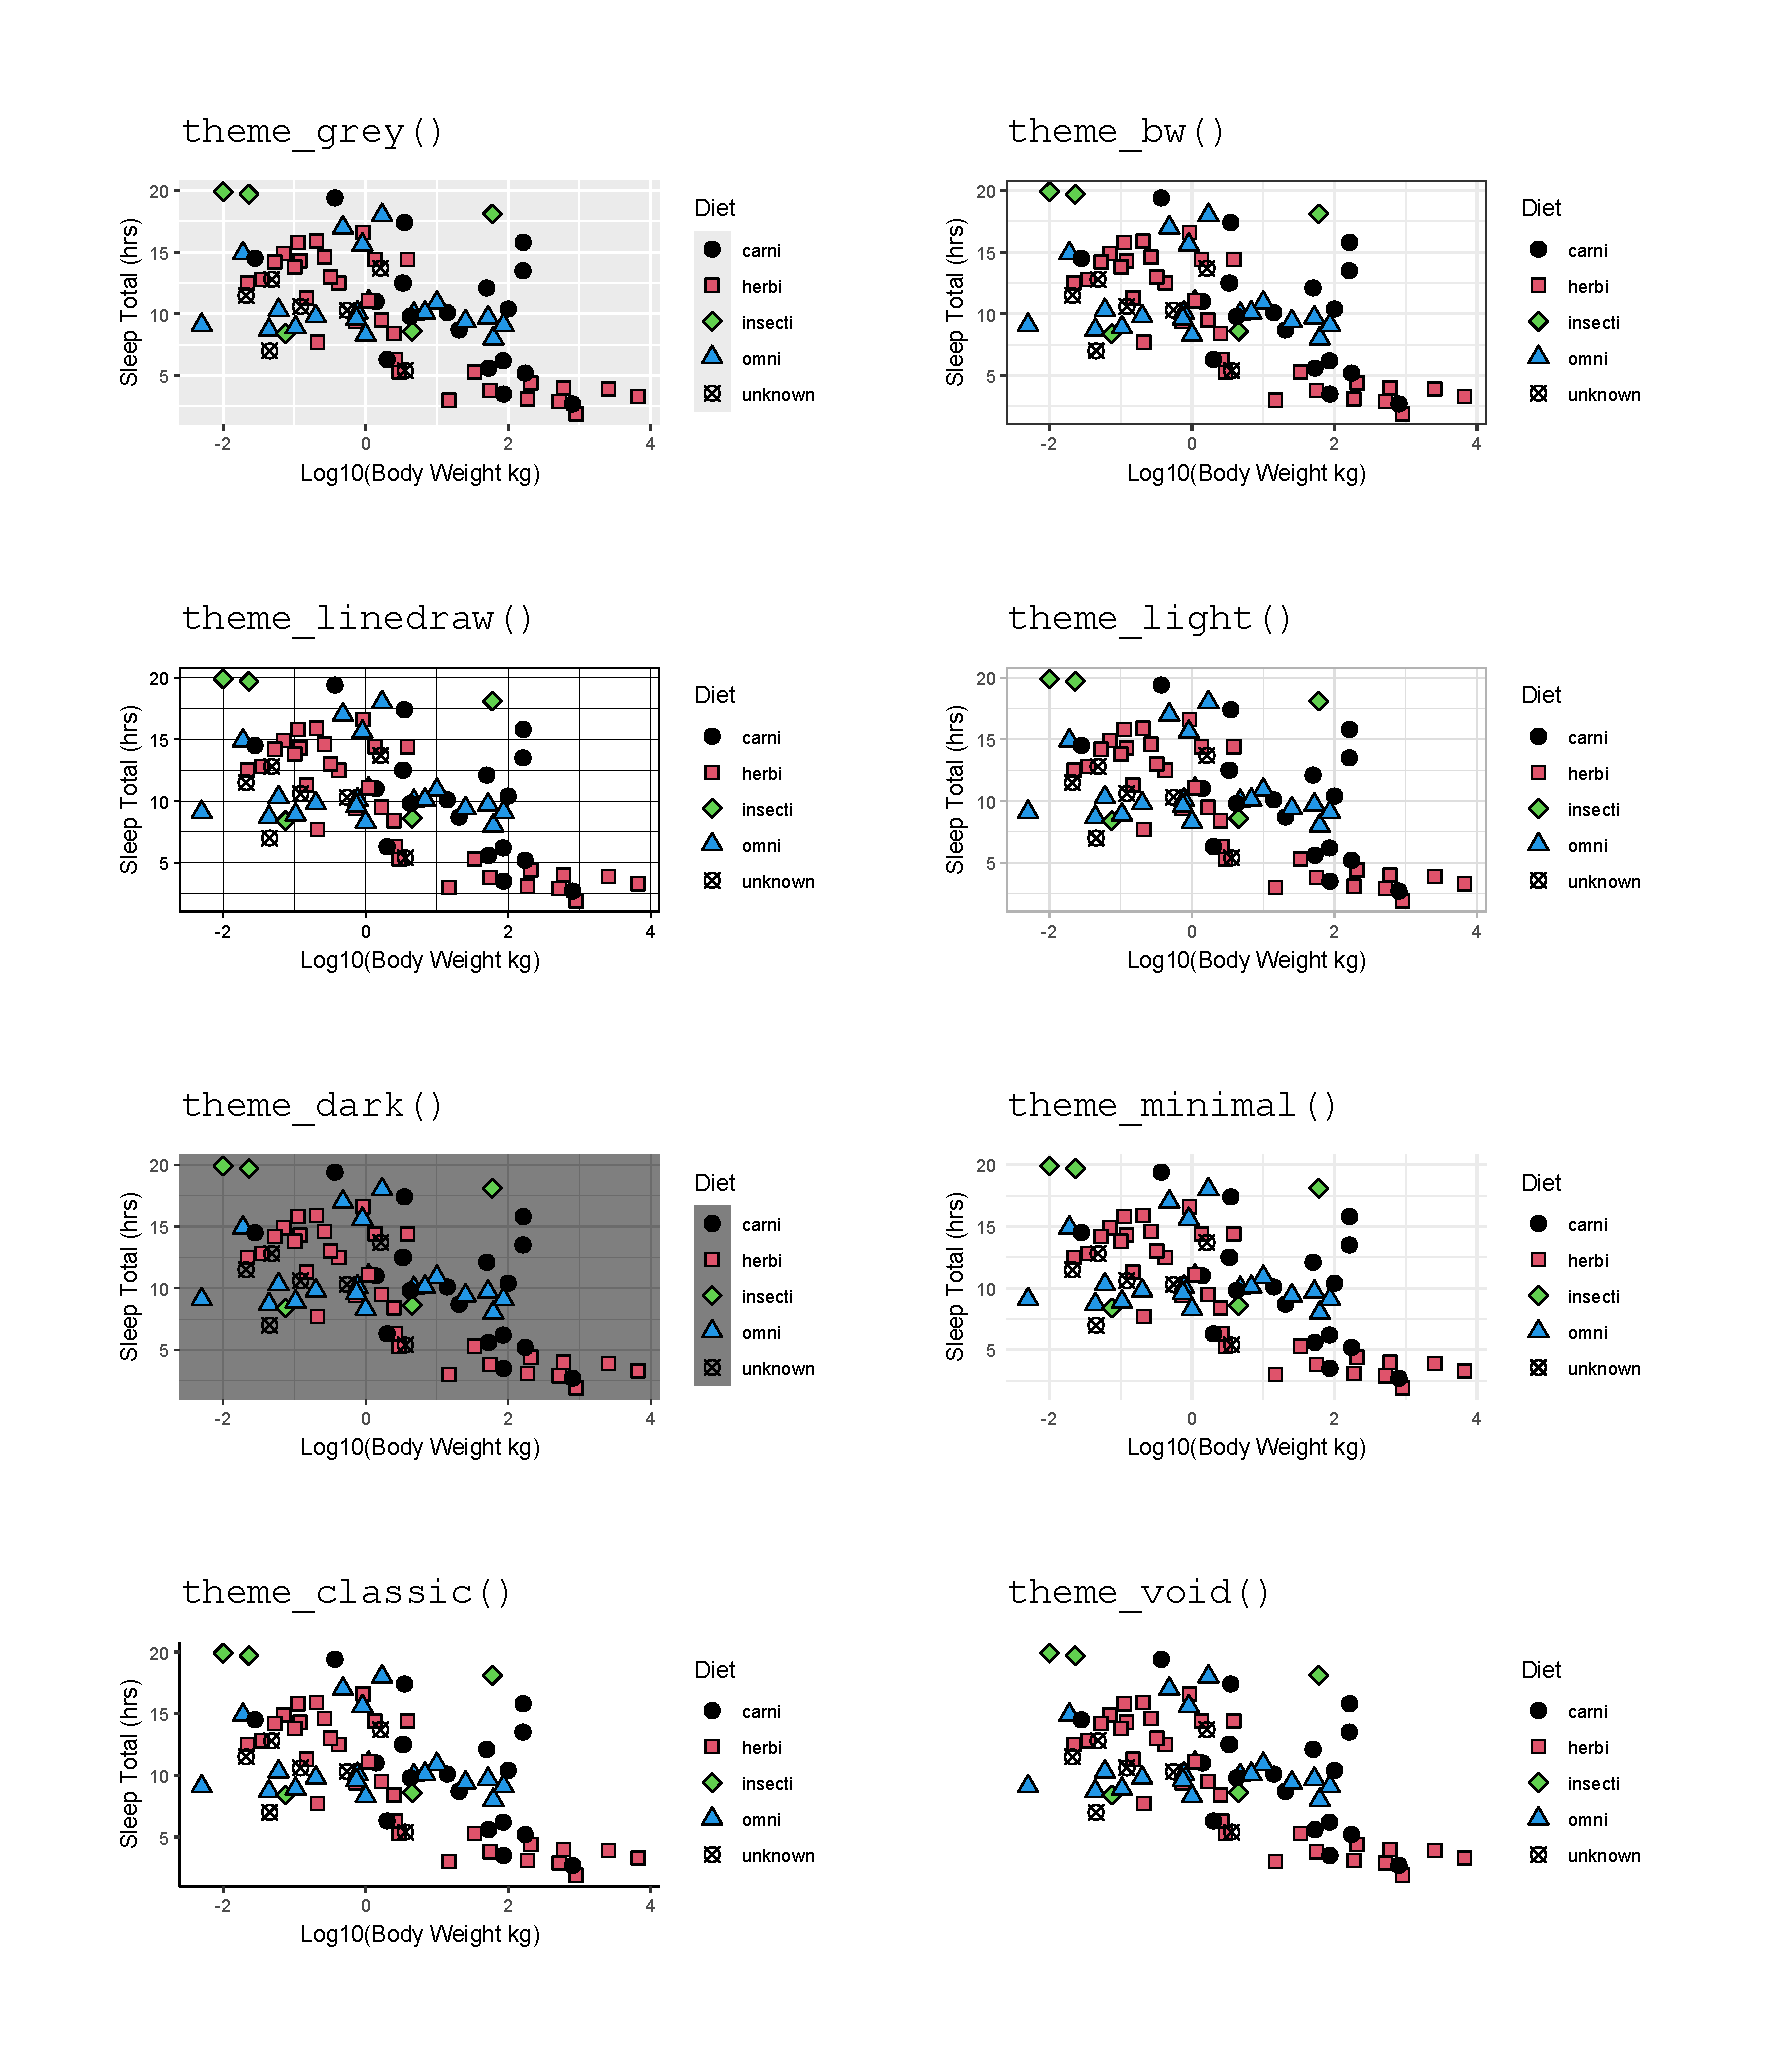
\includegraphics[scale = .35]{graphics/ch2Figs/ggEx_themes.pdf}}
\caption{Visual examples of the eight built-in themes \textit{ggplot2} provides.}
\label{fig:gg_built-in-themes}
\end{figure}

\vspace{1em}

\subsection{Customizing Themes}

Obtaining a more fine-grained control over the visual elements will require the use of \textit{ggplot2}'s \R{theme()} function. Admittedly, there is so much customization possible here that an exhaustive explanation would require at least an additional chapter's worth of content. For simplicity, we will restrict the discussion to axis text modifications. This should illustrate the overall process well-enough and generalize nicely across the plot's numerous other elements. That being said, readers looking to adjust these other elements will still need consult documentation of some kind for specifics. The official \textit{ggplot2} manual is unquestionably the best resource in this respect:

\begin{center}
\url{https://ggplot2-book.org/themes.html#sec-theme-elements}
\end{center}

To modify the axis text, we first need to specify, within the \R{theme()} function, the name of the element we want to modify. In this case, since we want to modify \textit{both} the x and y axis, we will specify \R{axis.text}.  Then we need to specify a function to modify this element we have chosen. In this case, since we want to modify text, we will use the function \R{element\_text()}. Within that, we can specify numerous arguments related to the text. For a full list of arguments, it is highly recommended that the reader consult the R documentation: \R{?element\_text()}

\begin{inR}
my_plot + theme_bw() +
  theme(
    axis.text = element_text(size = 18, face = "bold", colour = "red", angle = 45)
  )
\end{inR}

\vspace{2em}

\begin{figure}[H]
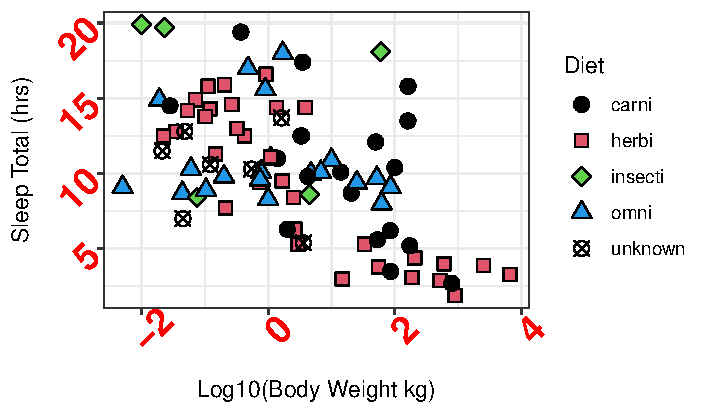
\includegraphics[scale = .75]{graphics/ch2Figs/ggEx_33.pdf}
\end{figure}

Notice that the code affected both axes; however, if we want to affect a change for only one axis (e.g., the x-axis) we just specify the element as \R{axis.text.x}.  This will also allow us to include a \R{margin} argument to affect the spacing around the text.

\begin{inR}
my_plot + theme_bw() +
  theme(
    axis.text.x = element_text(
      size = 18, face = "bold", colour = "red", angle = 45,
      margin = margin(t = 1, r = 0, b = 0, l = 0, unit = "cm")
    )
  )
\end{inR}

\vspace{2em}

\begin{figure}[H]
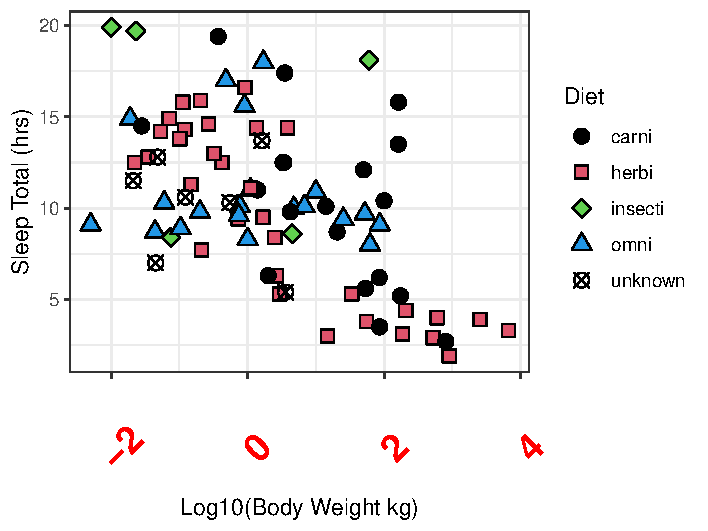
\includegraphics[scale = .75]{graphics/ch2Figs/ggEx_34.pdf}
\end{figure}

A similar logic applies to the axis title.  In that case we would modify the \R{axis.title} element. And again, if we wanted to modify the x-axis title specifically, we would use \R{axis.title.x}.  The y-axis title would of course be \R{axis.title.y}.

\begin{inR}
my_plot + theme_bw() +
  theme(
    axis.text.x = element_text(
      size = 18, face = "bold", colour = "red", angle = 45,
      margin = margin(t = 1, r = 0, b = 0, l = 0, unit = "cm")
    ),
    axis.title.y = element_text(
      size = 18, face = "italic", colour = "deepskyblue3", angle = 90
    )
  )
\end{inR}

\vspace{2em}

\begin{figure}[H]
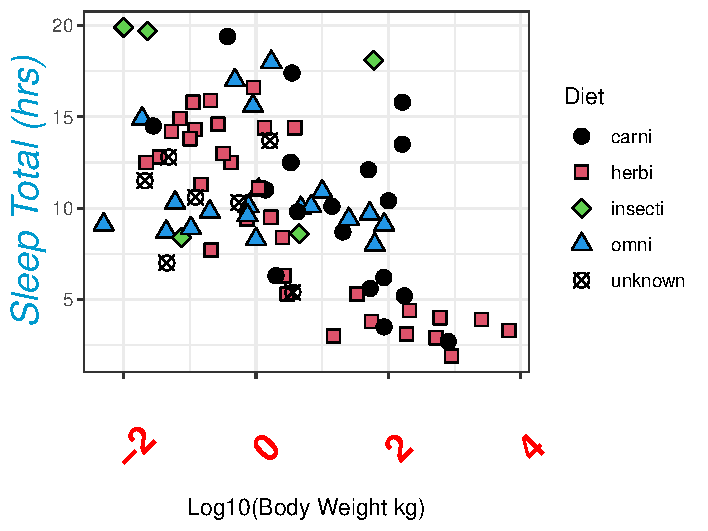
\includegraphics[scale = .75]{graphics/ch2Figs/ggEx_35.pdf}
\end{figure}

\section{A Final Note}

In the plots created above, we have gone through how to adjust a wide variety of elements but there are two adjustments that have not been discussed:

\begin{enumerate}
    \item How do you change the order of the categories?  For instance, suppose we wanted ``herbi'' to be at the top of the ``Diet'' legend. Or suppose we wanted it to come first in our sequence of faceted plots we created in section \ref{sec:facets}. How can we make that happen?
    \item  How do we adjust the names of the categories? Each category of vore/diet has had its name shortened, but what if we wanted to write out each category in its entirety. E.g., display ``carnivore'' instead of ``carni'', and ``herbivore'' instead of ``herbi'', and so on.
\end{enumerate}

The answer to both these questions requires first understanding ``factors,'' which will be explained later in the next chapter.